\documentclass[a4paper]{article}
%\documentclass[11pt,a4paper]{report}
%\documentclass[a4paper]{scrbook}

% definitions
\def\D{\partial}
\def\a{\alpha}
\def\dd{\displaystyle}
\def\ke{{k- \varepsilon}}
\def\e{\varepsilon}
\def\12{{\frac{1}{2}}}
\def\e{\varepsilon}
\def\ub{\bar{u}}
\def\vb{\bar{v}}
\def\wb{\bar{w}}
\def\pb{\bar{p}}
\def\up{{u}^\prime}
\def\vp{{v}^\prime}
\def\wp{{w}^\prime}
\def\pp{{p}^\prime}
\def\sij{\bar{S_{ij}}}
\def\de{\delta}
\def\ret{Re_{\tau}}
\def\uij{\overline{u_iu_j}}
\def\vij{\overline{v'_iv'_j}}
\def\vik{\overline{v'_iv'_k}}
\def\vjk{\overline{v'_jv'_k}}
\def\uv{\overline{v'_1v'_2}}
\def\vw{\overline{v'_2v'_3}}
\def\uw{\overline{v'_1v'_3}}
\def\uu{\overline{v_1^{\prime 2}}}
\def\vv{\overline{v_2^{\prime 2}}}
\def\ww{\overline{v_3^{\prime 2}}}

\usepackage[colorlinks=true,linkcolor=blue,anchorcolor=blue,urlcolor=blue,citecolor=blue]{hyperref}


\def\solidline{{$\textcolor{blue}{\overline{\hskip 0.5cm}}\ $}}
\def\dashedline{{$\textcolor{red}{\overline{\hskip 0.1cm}\ \overline{\hskip 0.1cm}\ \overline{\hskip 0.1cm}\ }$}}
\def\dashdottedline{$\overline{\hskip 0.1cm}\ \overline{\hskip 0.03cm}\ \overline{\hskip 0.1cm}\ $}
\def\dottedline{$\overline{\hskip 0.04cm}\ \overline{\hskip 0.04cm}\ \overline{\hskip 0.04cm}\ $}




%\setlength{\headheight}{ 27.8pt}
\usepackage{color}
\usepackage{subfigure}
\usepackage{graphicx,psfrag}
\usepackage[export]{adjustbox}
\usepackage[utf8]{inputenc}
\usepackage{amsmath}
\usepackage{amsfonts}
\usepackage{latexsym}
\usepackage{amssymb}
\usepackage[outdir=./]{epstopdf}
\usepackage{grffile}
\usepackage{url}
\usepackage{amssymb}
\usepackage{multirow}
\usepackage[intoc]{nomencl}
\makenomenclature
\usepackage[nottoc]{tocbibind}
\usepackage[toc]{appendix}
%\usepackage{subcaption}


%\usepackage{\mathaccent}
%% This will add the subgroups
%----------------------------------------------
\usepackage{etoolbox}
\renewcommand\nomgroup[1]{%
  \item[\bfseries
  \ifstrequal{#1}{A}{Latin symbols}{%
  \ifstrequal{#1}{B}{Greek symbols}{%
  \ifstrequal{#1}{C}{Brackets, Superscripts, Sub-scripts}{}}}%
]}
%----------------------------------------------

%% This will add the units
%----------------------------------------------
\newcommand{\nomunit}[1]{%
\renewcommand{\nomentryend}{\hspace*{\fill}#1}}
%----------------------------------------------

\def\karm{von  K\'arm\'an }

\pagestyle{myheadings}
\renewcommand{\subsectionmark}[1]{\markright{\thesubsection. #1}}
\renewcommand{\sectionmark}[1]{\markright{\thesection. #1}}


\begin{document}
%\title{MTF065 Turbulent Flow: An Example of a Report}

\title{Turbulent channel flow tests}
%\author{L. Davidson \\
%Division of Fluid Dynamics,
%Department of Applied Mechanics\\
%Chalmers University of Technology, G\"oteborg, Sweden\\
%\href{http://www.tfd.chalmers.se/\textasciitilde lada/}
%{\tt http://www.tfd.chalmers.se/\textasciitilde lada/}\\
%}

\maketitle
\thispagestyle{empty}

\cleardoublepage
%\thispagestyle{empty}
\pagenumbering{roman}
\newpage
%\section*{Channel Flow tests}
%
%The idea for this investigation is to check the cause for non-existant eddy viscosity in the channel for the ${Re_{\tau}} = 395$.
%We would perform two set of simulations on the mesh resolution 192x64x96 (Mesh1). We would write out all the quantities i.e. gradients $\frac{\D v_i}{\D x_i}$ , strain rates contraction and the traceless tensor formulated with the square of the velocity gradient tensor. In short, it would be same as we did previously in the poiseuille flow simulations and the Taylor green vortex simulations. \\

%{\bf i. Mesh 1 AA2016Wale}. We will perform the simulation for total 300,000 time steps and write out the data only for the $300,000^{th}$ time-step. In this tests we will not perform any kind of averaging, but write out all the details as discussed above. The idea here is to observe the order for the different quantities written out and to estimate the orgin of the error.\\
%
%{\bf ii. Mesh 1 AA2016Wale -  smaller perturbation number ($\epsilon$)}. Here we will perform the same simulation as above, but with the smaller $\epsilon$ added to make the system well-poised.
%The definition of which is as follows:\\
%%
%\begin{equation}
%\label{eddy-viscosity}
%\begin{split}
%{\nu_t} &= \left({C_w}{\Delta}\right)^{2}
%\frac{\left({S_{ij}^{d}}{S_{ij}^{d}}\right)^{3/2}}{\left(\sij \sij\right)^{5/2} + {\left({S_{ij}^{d}}{S_{ij}^{d}}\right)^{5/4}} + \epsilon}
%\end{split}
%\end{equation}
%%
%\\
%where, $\epsilon$ in our case is of the order $\sim 10^{-8}$.\\
%
%In this simulation we will change the value of $\epsilon$ to $\sim 10^{-30}$ or lower as the order of the terms in the numerator and the denominator are in between $\sim 10^{-18}$ to $\sim 10^{-25}$. Adding the epsilon of $\sim 10^{-8}$ in the denominator, which is relatively a larger number, is the reason we do not see the eddy viscosity in the channel. The purpose of this test is to see if we get the same orders of magnitude of the eddy viscosity as obtained in the tests performed using Matlab.
%\subsection{Discussion $9^{th}$ May}
%
%{\bf I. Test 1}. Here we have to improve the conditioning for the eddy viscosity in a more general way, rather than adding a constant  approximately. The idea as discussed by professor is as follows:
%\begin{equation}
%\label{eddy-viscosity-conditioning}
%\begin{split}
%A^{3/2} &= \left({S_{ij}^{d}}{S_{ij}^{d}}\right)^{3/2},\\
%A^{5/4} &= \left({S_{ij}^{d}}{S_{ij}^{d}}\right)^{5/4},\\
%B^{5/2} &= \left(\sij \sij\right)^{5/2}
%\end{split}
%\end{equation}
%When terms of the equation ~\ref{eddy-viscosity-conditioning} are replaced in the equation for ~\ref{eddy-viscosity} it looks as follows (not considering $\epsilon$ now):
%\begin{equation}
%\label{eddy-viscosity-changed}
%\begin{split}\\
%{\nu_t} &= \left({C_w}{\Delta}\right)^{2}
%\frac{A^{3/2}}{B^{5/2} + {A^{5/4}}},\\
%{OP} &= \frac{A^{3/2}}{B^{5/2} + {A^{5/4}}}\\
%\end{split}
%\end{equation}\\
%Now in the equation ~\ref{eddy-viscosity-changed} let's divide by ${A^{5/4}}$ and ${OP}$ would like:
%\begin{equation}
%\label{some_modification}
%\begin{split}\\
%{OP} &= \frac{A^{3/2}A^{\--5/4}}{\left(B^{5/2}\// {A^{5/4}}\right) + 1}\\
%\end{split}
%\end{equation}\\
%Some sort of this modification can give a general conditioning of the eddy viscosity.\\
%{\bf II. Channel flow}.  Pressure and the density are negative i.e. mass deficit in the channel\\
%{\bf III. Taylor green vortex}. Finer resolution with changed value of $\epsilon$. %%
%\begin{equation}
%\label{some_modification}
%\begin{split}
%{OP} &= \frac{A^{1/4}}{\left(B^{1/2}\// {\left(A^{1/4} + 10^{-10}\right)}\right)^{5} + 1}
%\end{split}
%\end{equation}\\
%%Some sort of this modification can give a general conditioning of the eddy viscosity.\\
%%{\bf II. Channel flow}.  Pressure and the density are negative i.e. mass deficit in the channel\\
%%{\bf III. Taylor green vortex}. Finer resolution with changed value of $\epsilon$. 
%
%\subsection{Next steps $15^{th} May$}
%
%Since the reason for the missing eddy viscosity is found, $\epsilon$ = $10^{-30}$, and an appropriate wale model co-efficient, $C_{W} = 0.55$, we should start the wale model simulations on the channel flow.
%\\
%\\
%{\bf i}. AA2016Wale and OneWale\\
%{\bf ii}. AA2016wale with double precision. This will be a comparison to see if any significant changes are present in the flow.


\newpage
\thispagestyle{empty}
\listoffigures

\newpage
\thispagestyle{empty}
\listoftables

\newpage

\nomenclature[A, 01]{$L_x$}{Length of the domain, stream-wise direction}
%  \nomunit{$6.67384 \times 10^{-11}\, N \cdot m^2/kg^2$}}
\nomenclature[A, 02]{$L_y$}{Height of the domain, wall-normal direction} 
%  \nomunit{$299,792,458\, m/s$}}
\nomenclature[A, 03]{$L_z$}{Width of the domain, span-wise direction}
%  \nomunit{$6.62607 \times 10^{-34}\, Js$}}
\nomenclature[A]{$U$}{Mean stream-wise velocity}
\nomenclature[A]{$V$}{Mean wall-normal velocity}
\nomenclature[A]{$W$}{Mean span-wise velocity}
\nomenclature[A]{$u$}{stream-wise velocity fluctuation}
\nomenclature[A]{$v$}{wall-normal velocity fluctuation}
\nomenclature[A]{$w$}{span-wise velocity fluctuation}
\nomenclature[A]{$\ub$}{filtered stream-wise velocity}
\nomenclature[A]{$\vb$}{filtered wall-normal velocity}
\nomenclature[A]{$\wb$}{filtered span-wise velocity}

%%% Greek %%%
\nomenclature[B, 04]{$\de$}{Half-channel height, wall-normal direction}
\nomenclature[B, 03]{$\mathbb{R}$}{Real Numbers}
\nomenclature[B, 02]{$\mathbb{C}$}{Complex Numbers}
\nomenclature[B, 01]{$\mathbb{H}$}{Quaternions}

%% Bracket %%
\nomenclature[C]{$V$}{Constant Volume}
\nomenclature[C]{$\rho$}{Friction Index}
 


\printnomenclature

\newpage
\thispagestyle{empty}
\cleardoublepage
\tableofcontents


\thispagestyle{empty}
\pagenumbering{arabic}
\newpage

%\chapter{Introduction}
\section{Introduction}
Navier-stokes equations (NS) are the governing equation for the fluid flow. The flow of fluid can be termed as laminar or turbulent depending on the dimensionless Reynolds (Re) number. Reynolds number of a flow gives the measure of the relative importance of the inertia force over the viscous force. When the viscous forces are dominating i.e. the Re no is small the flow is laminar. Any disturbance present or originating in the laminar flow would be damped out by the viscosity. Above a certain value of Re number the flow becomes turbulent i.e. inertia forces are quite significant and any disturbance or irregularity would be amplified resulting in the flow becoming random and chaotic with the velocity and the pressure changing continuously in time and with in the substantial region of the flow i.e. turbulent regime. 

Turbulent flows comprise of the rotating flow structures called turbulent eddies. These structures posses a wide range of length scales. The largest eddies interact with the mean flow and derive the energy from it. These large eddies are anisotropic and are affected by the inertia forces. They are insensitive to the viscosity. These eddies than transfer the energy further to the smaller and the smaller eddies via a mechanism called energy cascade. The energy present in the smaller eddies is dissipated by working against the viscous forces.

Analytical solution of the flow governing equations are only available for certain basic cases viz. Couette flow or Poiseuille flow. The solution for the flow involving turbulence or with complex boundary conditions is not available. Thus the equations have to be solved numerically i.e. numerical simulations. The most straightforward approach for the solution of the turbulent flows is to perform Direct numerical simulation (DNS), where the flow governing equations are discretized and solved numerically. This approach resolves all the existing scales in the flow which eventually results in a computationally expensive simulation. With the latest advancement in the computational resources this approach is applicable only to flows with smaller to moderate Reynolds number (see section). The remedy to this problem is not to resolve all scales of motion present in the flow. This alternative approach is turbulence modeling. In this approach the entire scales of motion present in the flow are modeled, Reynolds averaged Navier stokes equation (RANS), or a certain level of scales are chosen to be resolved and the rest are modeled, Large eddy simulation (LES). 

A sophisticated approach to obtain the solution of the turbulent flows is to use the Reynolds decomposition, where the flow properties are decomposed in to their respective mean and fluctuating parts, in combination with the flow governing equations to obtain the RANS equations. RANS equations describe the evolution of the mean flow properties. An additional term is obtained in RANS equations which represents the effects of the turbulent fluctuations i.e. fluctuating velocity components. This additional term has to be modeled to close the set of equations. 

In LES large scales are resolved and the smaller scales are modeled. The separation of the scales is achieved by a filtering process (see section). Using the filtering operation, where the flow properties are decomposed in to resolved/filtered and unresolved/residual part, in combination with the NS equations we get the LES equations. These equations describe the evolution of the filtered quantities. Additional term is obtained in the LES equations which represents the effect of the residual scales on to the filtered scales. This additional term has to be modeled to close the set of equations.

In terms of the computational expense LES lies in between the solution of turbulent flows by DNS and RANS. This method is motivated by the limitations of the RANS and the DNS approach \cite{pope:book}. LES involves modeling of the smaller scales of motion and does not resolve the entire range of scales as done in DNS. This allows this method to be applicable to flows with high Reynolds number. In comparison to RANS, where the entire range of scales is modeled, LES models only the smaller scales and thus it is computationally expensive. This extra computational overhead is justified when an accurate and reliable prediction of the flow is obtained. Specifically in the flows where the unsteadiness due to the larger scales are important i.e. flow over the bluff bodies LES is the appropriate choice. With the recent developments in the computational resources a lot of research is going on to make LES applicable to complex geometries and industrial flows.

\textbf{\emph{Why LBM?}}\\
A wide variety of methods are available to find the solution to the fluid flow equations. These methods differentiate from each other on the basis of the level of description of the fluid i.e microscopic, mesoscopic  or macroscopic. The methods are grouped under two terminologies: Conventional methods and the particle based methods~\cite{krueger:book}. The former methods assumes the macroscopic description or continuum approach of the fluid viz. finite difference method, finite volume method. The latter assumes the microscopic or mesoscopic description viz. Molecular dynamics, LBM etc. In this work, LBM has been chosen to perform the LES of the wall-bounded turbulent flow. This method differentiates from the conventional methods in the sense that it does not solve the flow equations directly, but it solves the boltzmann equation. Well known methods exist that can relate the dynamics of this equation to the macrosccopic conservation equations~\cite{krueger:book}. 

Because of its kinetic nature the LBM enjoys several advantages over other numerical methods and that makes it a lucrative option for the simulation of the fluid flow~\cite{doolen}. \emph{S. Chen et. al}~\cite{doolen} points out some major advantages of LBM over other methods:

\begin{itemize}
\item The convection operator (streaming process) of LBM is linear. This behavior is in contrast to the non-linear behavior of the convection term in the conventional methods that use the macroscopic description. Streaming process in combination with the relaxation process (collision operator) is able to recover the non-linear convection behavior present in the macroscopic equations.

\item The pressure of the LBM is computed from the equation of state. On the other hand, a poisson equation has to be solved for the pressure in the conventional methods which is quite tedious to discretize and solve numerically.

\item The LBM discretises the Boltzmann equation in velocity space and only retains a minimal set of particle velocities that are needed to recover the proper macroscopic behaviour. This makes the LBM considerably more computationally efficient than other particle-based methods~\cite{thesis:bespalko}.

\item In a grid, the collision process is local to each node and the interaction between the nodes is linear. It is this property of LBM which makes it very amenable to high performance computing on parallel architectures including GPU`s ~\cite{krueger:book}.
\end{itemize}

All methods have their advantages and disadvantages and there is no one method that is superior to other methods. LBM has also disadvantages: it memory intensive~\cite{krueger:book}, not efficient for steady flow simulations~\cite{geller}, it is limited to incompressible problems~\cite{thesis:bespalko} etc. It is a relatively young method and is evolving at a fast pace, which means that the applicability of the method to variety of problem is still increasing~\cite{krueger:book}.


\subsection{Literature survey}


\subsection{Objectives and Motivation}


%\newpage

\newpage

\section{Lattice Boltzmann theories}

\newpage

\section{Turbulence theories}
\subsection{RANS}
\subsection{LES}

\newpage

\section{Implementation}
The WALE model has been implemented initially in the D3Q27 Matrix code developed in the Institute of Computational modelling in Civil Engineering. This code uses two set of arrays to store the distribution functions and to exchange the post-collision distribution functions every time-step. The WALE model implementation requires the computation of the strain rate tensor and the vorticity rate tensor, which requires the information of the velocity gradients. The velocity gradients have been computed using the finite differences. The macroscopic velocity computed from the distribution functions are used to compute the velocity gradients in every time-step. Apart from the WALE model implementation the topic on the conditioning of the WALE model equation will be discussed here. Towards the end of the section the numerical results of the Taylor green vortex simulations will be compared to the analytical solution to confirm the validity of the eddy-viscosity obtained from the WALE model.

\subsection{Discretisation}
Several velocity gradients i.e. $\partial u_i/\partial x_i$ and $\left(\partial u_i/\partial x_j + \partial u_j/\partial x_i\right)$ are directly available from the Cumulant LB solver~\cite{geier:parameter}. The computation of the strain rate tensor can be easily carried out with those available gradients. But the available information of the velocity gradients was not enough to compute the rotation rate tensor i.e. $\left(\partial u_i/\partial x_j - \partial u_j/\partial x_i\right)$. Since the vorticity calculations had to be  performed using the finite difference method, it was decided to compute the velocity gardients using the finite difference method. \emph{Weickert et.al}~\cite{weickert:LES} implemented the WALE model in the MRT LB framework and they have computed the velocity gradients using the finite differences. 

The purpose of the SGS models is to dissipate the resolved turbulent fluctuations~\cite{davidson}. When finite differences are used in combination with the LES method great care has to be taken to choose the non-dissipative finite difference scheme. This is done to avoid the masking effect of the numerical dissipation on to the dissipation introduced by the SGS models. Taking that into consideration a central difference scheme was chosen to compute the velocity gradients.\\\\
%
\textbf{Treatment of velocity gradients near the boundaries}

In order to avoid the fluid nodes, near the boundaries, accessing the non-fluid nodes due to the central differencing, forward differences and backward differences were used at the respective boundaries to compute the velocity gradients. Fig.(\ref{Finite differences bound}) shows a cuboid marked with the red dots at the inlet, front and the bottom face. The first set of fluid nodes near these faces use forward difference to compute the velocity gradients and the first set of fluid nodes at the exit, top and back faces use backward differences to compute the gradients along the respective directions. Rest fluid nodes used central differences.

\begin{figure}[b]
\centering
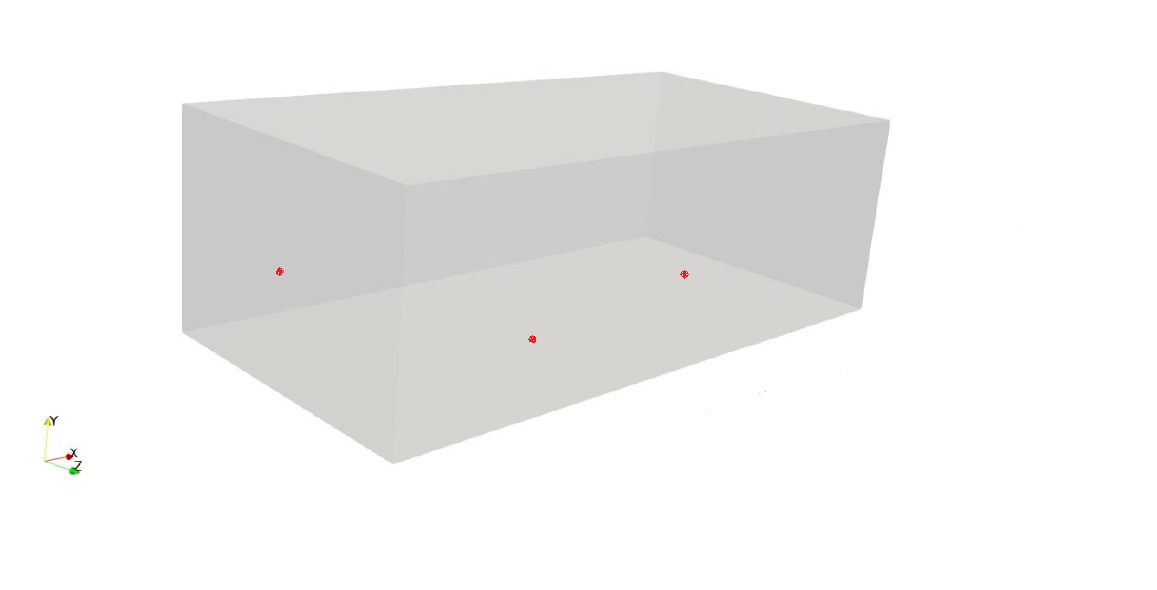
\includegraphics[width=8cm]{04_Implementation/figur/3D_Domain_gradients.png}
\label{Finite differences bound}
\caption{Cuboid representing a channel}
\end{figure}
\subsection{Implementation of eddy viscosity contribution}

The WALE model has been implemented in the LB kernel itself "LB\_Kernel\_2SOD". Few other variations were tried but they required thread synchronisation which is not optimal to do in terms of the efficiency. Hence, it was implemented in the kernel itself. An additional viscosity called eddy viscosity $\left(\nu_t\right)$ has to be introduced in to the solver to model the turbulence. This is given by:
%
\begin{equation}
\label{Eddy viscosity}
\nu_t = \left(C_W \Delta_x \right)^2 \overline{OP}
\end{equation}
\subsection{Taylor-Green vortex simulations}
%
where $C_W$ is the model constant and is
\begin{figure}[h]
%\centering
\begin{minipage}[b]{0.5\textwidth}
\subfigure[global coordinates]{
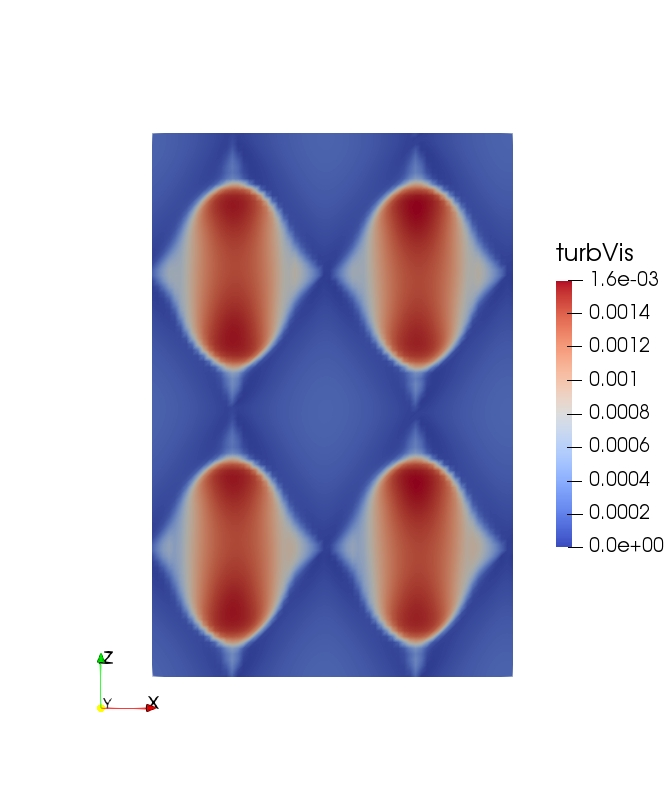
\includegraphics[width=6.7cm]{04_Implementation/figur/nutSimulation_latex_64.jpg}}
\end{minipage}
\end{figure}
%


\newpage
%\chapter{Model set-up and theories}

\section{Model set-up and theories} 
Apart from the free shear flows, most turbulent flows are bounded by one or more solid surfaces depending on whether they belong to class of the internal or external flow of fluids i.e. flow through pipes and flow over a car respectively.  In this investigation one of the simplest internal flow has been chosen for the validation \& testing of the implementation: fully developed channel flow. This flow is considered to be of prime importance as it has played a prominent role in the development of the study of the wall bounded turbulent flows~\cite{pope:book}.~\cite{pope:book} has described the fundamental theories of the full developed channel flow in great detail. ~\cite{froehlich:book} also has a good compilation on the fully developed channel flow. 

In this section a brief description of the turbulent channel flow with some basic theories is presented. Later on it is followed by description of the computational domain, meshing, initial conditions, boundary conditions, pressure gradient modelling, solver settings and in the end by post-processing. 

\subsection{Turbulent channel flow} \label{validation}

Fully developed turbulent channel flow is a classic benchmark case and has been studied extensively to investigate and understand the mechanics of wall-bounded turbulent flows. It is the geometrical simplicity of this case that has lured to a large number of, computational (DNS) and experimental, investigations being carried out for the turbulent channel flow over the years and as a result, an adequate database (DNS data) for certain Re-numbers is already available~\cite{channeldata:99}. Historical progression in the turbulent channel flow simulations have been very well documented in the literature by \emph{Kim et al.}~\cite{kim:moin:moser:87}. Also, Kim has pointed out several difficulties related to the experimental measurements and how numerical simulations serve as an essential tool, alongside the experimental results, for the study of the wall-bounded turbulence. The recent development along with the comparison of the DNS results of the turbulent channel flow simulations for higher Re-numbers is documented in ~\cite{lee:moser:15}.\\
%
\begin{figure}[h]
    \centering
    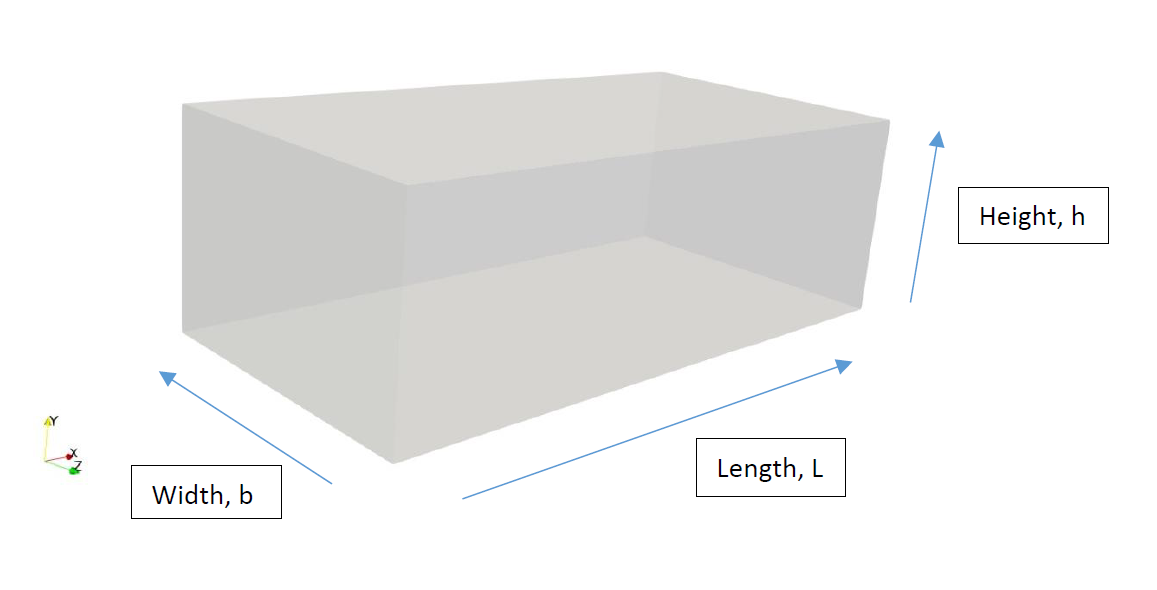
\includegraphics[width=0.8\textwidth]{figur/3D_Domain.png}
    \caption{3D rectangular duct}
    \label{3D domain}
\end{figure}
%
As shown in figure \ref{3D domain}, a 3D rectangular duct has been chosen as the computational domain. The positive x-axis is the stream-wise direction or the flow direction with the flow varying in the y-direction, the height $h = 2\de$, the wall-normal direction. The z-axis is the span-wise direction, the width b. The domain is long and has a large aspect ratio $\left(b/\de \gg 1\right)$. The bottom (y = 0) and top (y = $2\de$) surfaces of the domain are walls. The mid-plane (y = $\de$), which is frequently termed as the half-channel width in the literature, is ambiguous with the assigned Cartesian coordinate directions in this case and hence term half-channel height will be used(h = $\de$). 

The mean velocities in the three directions are $U$, $V$, $W$, the stream-wise, wall-normal and span-wise velocities, and the corresponding fluctuating velocities are $u$,$v$ and $w$. The mean span-wise or cross-stream velocity is zero, $W = 0$. 
In the turbulent channel flow test case, fully developed flow region in the channel is of our interest i.e. it is the region where the velocity statistics of the flow remain invariant to spatial changes, x-direction in our case. Also, the domain is large enough in the span-wise direction, z, compared to the half-channel height, $\de$, so that the flow remains statistically independent of the z-direction. In short, we have two homogeneous flow directions along x \& z-axis. Thus, the flow is said to be statistically one- dimensional as the flow statistics vary only in one-direction i.e. y-direction. 
%%
%\begin{figure}[h]
%    \centering
%    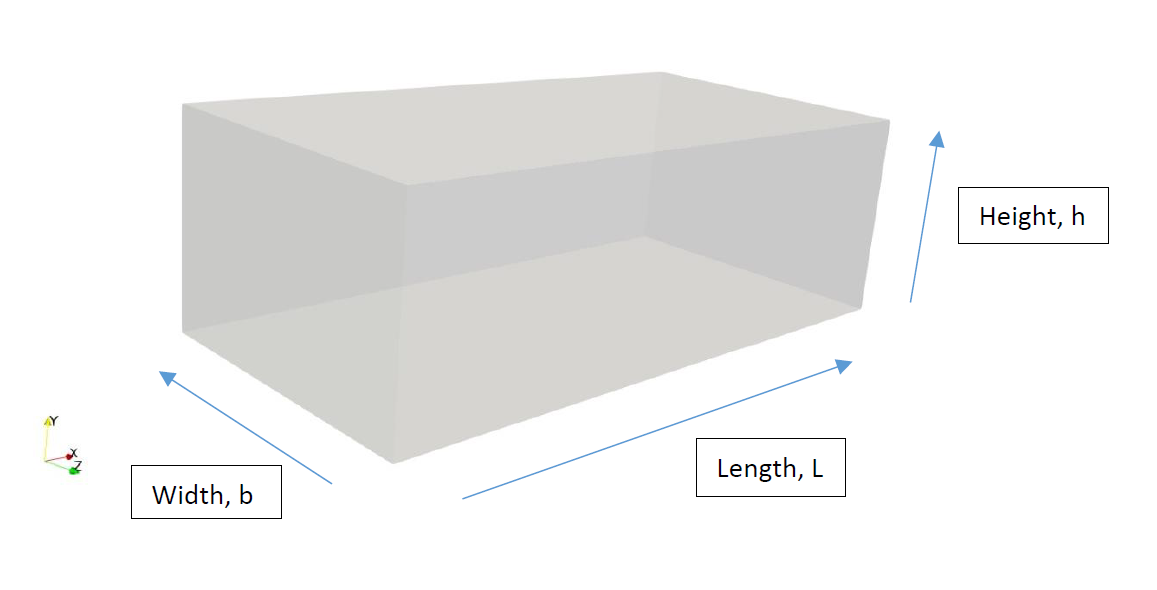
\includegraphics[width=0.7\textwidth]{figur/3D_Domain.png}
%    \caption{3D rectangular duct}
%    \label{3D domain}
%\end{figure}
%%


\subsubsection{Governing equations}

Turbulent channel flow is fully developed, where the velocity statistics along the stream-wise direction remain constant i.e. ${\D U}/{\D x}=0 $, and statistically one dimensional, where the flow statistics vary only in the wall-normal(y) direction. There is no mean flow in the span-wise direction i.e $W=0$ and thus the gradient of the span-wise velocity in the span-wise direction is zero i.e. ${\D W}/{\D z}=0 $. The mean continuity equation for the incompressible flow results in the mean wall normal velocity gradient to be zero:
\begin{equation}
\label{zero wall-normal mean vel. gradient}
\begin{split}
{\D V}/{\D y}&=0
\end{split}
\end{equation}
The eq.~\ref{zero wall-normal mean vel. gradient} when integrated, within the wall limits [0,$2\delta$], gives $V=const(y)$ and using the no-slip boundary condition, $U_i = 0$, applied at the walls results in $V = 0$. Now to satisfy the resulting continuity equation eq.~\ref{zero wall-normal mean vel. gradient}, $V$ has to be zero everywhere in the domain. Using the above made considerations and applying it to the mean stream-wise momentum equation we will have the following force balance:
\begin{equation}
\label{Forces channel flow}
\frac{\D \tau}{\D y} = \frac{\D P}{\D x}\\
\end{equation}
where $\tau = \left(\mu \frac{\D U}{\D y} - \rho\uij\right)$ is the total shear stress.\\

The eq.~\ref{Forces channel flow} shows that the total shear stress gradient and the pressure gradient balance each other in the full developed channel flow. It shows an equality of the form $\emph{f(x)}= \emph{g(y)}$ and for this equality to hold it is important that both $\emph{f(x)}$ and $\emph{g(y)}$ are individually constants. In eq.~\ref{Forces channel flow} both the gradients are dependent on different variables and thus they must be individually constants for this equality to hold. $$\frac{\D P}{\D x} = const\  \&\  \frac{\D \tau}{\D y} = const$$\\
%
Total shear stress is the summation of the viscous stress, $ \mu \frac{\D U}{\D y} $, and the Reynolds stress, $- \rho\uij$. At the wall with the no-slip boundary condition applied, the Reynolds stresses are reduced to zero and thus the shear stress near the wall or to be specific at the wall would entirely be dominated by the viscous stresses. At the walls the Reynolds stresses drop to zero and the stress at the walls can be defined as the \emph{wall shear stress},\marginpar{\bf wall shear \\stress} the region where the viscous stresses are dominant:
\begin{equation}
\label{Wall shear stress}
\begin{split}
\tau_w = \mu \frac{\D U}{\D y}\\
\tau\left(0\right) = \tau_w  = -\tau\left(2\delta\right)\\
\end{split}
\end{equation}\\
%
Now we can integrate the eq.~\ref{Forces channel flow}, from 0 to $2\delta$, for the pressure gradient and express the solution in terms of the $\tau_w$:
%
\begin{equation}
\label{Solution equations}
\begin{split}
-\frac{\D P}{\D x} = \frac{\tau_w}{\delta} \ ,\\
\end{split}
\end{equation}\\ 
%
From the fully developed channel flow it is known that the mean velocity profile (time-averaged) remains constant. It is clear from eq.~\ref{Wall shear stress} that wall shear stress is linearly proportional to the velocity gradient near the wall. A constant velocity profile implies that the wall shear stress will also be constant in a fully developed channel flow. Thus from eq.\ref{Solution equations} we can say that the pressure gradients is constant. Integrating the eq.~\ref{Forces channel flow}, from 0 to some y, with the no-slip boundary condition at the wall results in the following solution:
\begin{equation}
\label{Shear stress profile}
\begin{split}
\tau\left(y\right) = \tau_w \left(1 - \frac{y}{\delta}\right)\\
\end{split}
\end{equation}\\ 
%
It is this pressure gradient that drives the flow through the infinite parallel plates.The pressure gradient in eq.~\ref{Solution equations} is negative as the viscous effects decreases the pressure along the stream-wise direction.  For a given pressure gradient and the half-channel height we get a linear shear stress profile from eq.~\ref{Solution equations} and ~\ref{Shear stress profile} independent of the fluid properties and the state of the fluid motion (laminar or turbulent)~\cite{pope:book}.
Experimental and numerical results~\cite{kim:moin:moser:87} show that the total shear stress profile is anti-symmetric about the channel mid height $ y=\delta $ and thus $\tau\left(\delta\right) = 0$.
%
\subsubsection{Scaling units} \label{scaling}
The Reynolds stresses decreases towards the wall, remain zero at the wall and so does the eddy viscosity (\emph{Boussinesq hypothesis}). The value of the eddy viscosity ranges from zero, at the wall, to several orders of magnitude higher than the molecular viscosity, in the core region of the turbulent boundary layer~\cite{cengel:book}. From the figure. \ref{TFlow} it can be seen that the velocity profile changes more slowly (more flatter compared to the parabolic flow profile) in the core of the turbulent boundary layer, where the eddy viscosity is higher than the molecular viscosity, and there is an abrupt change in the velocity profile near the wall, where the molecular viscosity is dominant. The turbulent flow profile has the largest gradient near the wall. 
\begin{figure}[h]
    \centering
    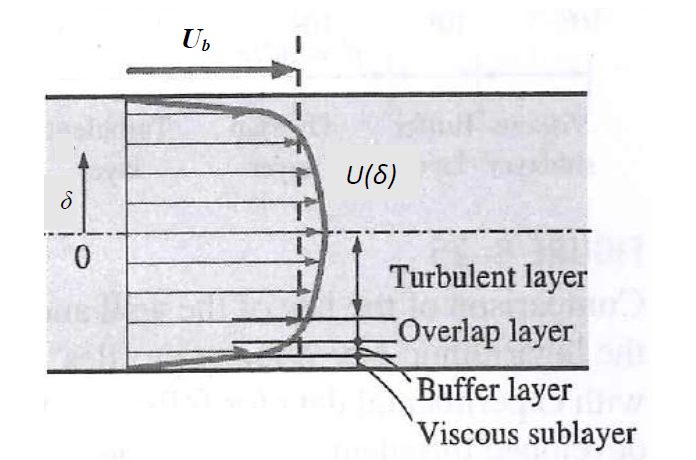
\includegraphics[width=0.6\textwidth]{figur/Turbulent_profile.png}
    \caption{Velocity profile in the fully developed channel flow ~\cite{cengel:book}}
    \label{TFlow}
\end{figure}

Turbulent flow along the wall can be considered to consist of four different layers, characterised by their distance from the wall. All four layers have been approximately shown in figure \ref{TFlow}. The layer closet to the wall is the viscous sub-layer, where the viscous effects are dominant. The velocity profile changes linearly with the distance from the wall and the flow is streamlined. Next to the viscous sub-layer is the buffer layer, where the turbulent stresses start to develop, but still the viscous stresses are dominant. Above the buffer layer is the overlap layer, where the turbulent stresses are significant, but still not dominant enough as the viscous stresses. The layer above the overlap layer for the rest of the flow is the outer or turbulent layer, where the turbulence stresses dominate over the viscous stresses.\\
%
A single analytical relation for the entire turbulent velocity profile is not suitable, as different regions or layers execute different flow characteristics. The best possible option is to find the key parameters or the functional forms using the dimensional analysis and later on experimental data can be used to obtain the numerical values of the any constants.\\

\textbf{i. Viscous sub-layer :} With the no-slip boundary condition applied at the wall, \emph{$u_i(0,t) = 0$}, the entire contribution to the shear stress is purely via viscous stresses i.e. $\tau_w$. From eq. \ref{Wall shear stress} it is clear that shear stress is proportional to the molecular viscosity. The thickness of this layer is very small, but it plays an important role on the flow characteristic because of the presence of large velocity gradients in it. The velocity profile remains linear in this layer and also it has been shown in certain experiments ~\cite{cengel:book}. Since the velocity profile is linear the gradient in the equation \ref{Wall shear stress} remains constant i.e. ${\D U}/{\D y} = {U}/{y} $. Thus the wall shear stress can be written as:
\begin{equation}
	\label{viscous sub-layer equ}
	\frac{\tau_w}{\rho} = \frac{\nu U}{y}
\end{equation}\\
Near the wall the important parameters are : $\tau_w$, $\rho$, $\nu$. The square root of the term on the left hand side has the dimensions of velocity and thus we define a new parameter as the \emph{\textbf{friction velocity}, $u_\tau$}:
\begin{equation}
	\label{friction velociy}
	u_\tau = \sqrt{\frac{\tau_w}{\rho}}
\end{equation}\\
Replacing $u_\tau$ in the eq. \ref{viscous sub-layer equ} we have \emph{\textbf{the law of wall}}:
\begin{equation}
	\label{law of wall}
	\frac{U}{u_\tau} =  \frac{u_\tau y}{\nu}
\end{equation}\\
The quantity $\nu / u_\tau $ has the dimensions of length and it is called \emph{\textbf{viscous length}} , $\delta_\nu$,  and it is used to nondimensionalze the distance from the wall, y. In the analysis of the boundary layer flow, it is convenient to work with the nondimensionalised distance and the velocity. The nondimensionalised quantities are represented with a $+$. \\
\emph{\textbf{Nondimensionalised variables} : } \begin{equation}
	\label{nondimensions}
	y^+ = \frac{y u_\tau }{\nu} \    and \    u^+ = \frac{U}{u_\tau}
\end{equation}\\
\emph{\textbf{Normalised law of the wall : }}\begin{equation}
	\label{nondimensions law of wall}
	u^+ = y^+ 
\end{equation}
This law shows a very good correlation with the experimental data for smooth surfaces for $0\leq {u_\tau y}/{\rho} \leq 5	$. Thus for the $y^+ =  5$ we will have the linear velocity profile in the viscous sub-layer. \\

\begin{figure}[t]
    \centering
    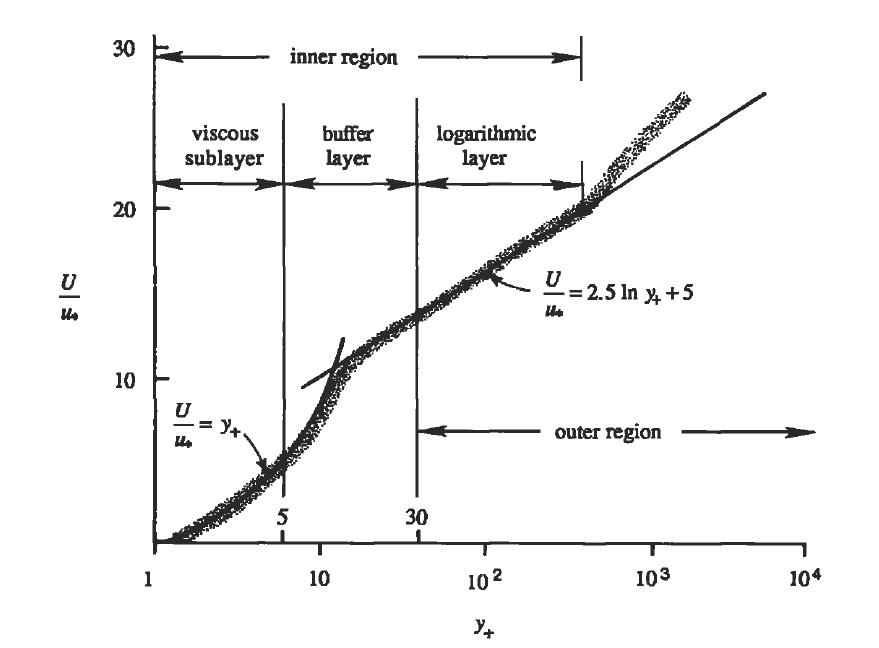
\includegraphics[width=0.9\textwidth]{figur/Log-law-plot.png}
    \caption{Nondimensional velocity $u^+$ vs. the nondimensional distance $y^+$ (plotted in logarithmic scale) ~\cite{kundu:book}}
    \label{log-log plot}
\end{figure}


\textbf{ii. Overlap layer:} From the dimensional analysis and the experimental results it proved that the velocity in the overlap region is proportional to the logarithm of distance and it can be expressed as: 
\begin{equation}
	\label{log law}
	u^+ = \frac{1}{\kappa}\ ln\ y^+ + \ B \ or \  u^+ = 2.5\ ln\ y^+ + \ 5.0 
\end{equation}
where $\kappa$ and $B$ are constants and equal to 0.40 and 5.0 respectively. The eq. \ref{log law} is called the \emph{logarithmic law} and the overlap layer is also called as the \emph{logarithmic layer} or \emph{log-law layer}. It is clear from the figure \ref{log-log plot} that the eq. \ref{log law} represents the experimental data quite satisfactorily from $y^+ \geq 30$ till outer region. Neither eq. \ref{log law} nor the eq. \ref{law of wall} represents the experimental data satisfactorily in the buffer layer.
From Figure. \ref{log-log plot} it is seen that :\\

\emph{\textbf{viscous sub-layer}	} : $y^+ \leq  5$ \\ 

\emph{\textbf{buffer layer}} : $y^+ \geq  5$ till $y^+ \leq  30$ \\

\emph{\textbf{logarithmic layer}} : $y^+ \geq  30$ till $y^+ \leq  10^3$ \\\\
%
\textbf{iii. Outer layer:} The velocity law for this region is:
\begin{equation}
	\label{vel defect law}
	\frac{\left(U_{max} - U\right)}{u_\tau} = \frac{1}{\kappa}\ ln\ \left(\frac{y}{\delta}\right)  
\end{equation}
The difference between the mean center line velocity, $U_{max}$, and the mean velocity, $U$ is called the \emph{\textbf{velocity defect}} and thus this law is called the \emph{\textbf{velocity defect-law}}. In this region the turbulent stresses are dominant compared to the viscous stresses and this is also seen from the eq. \ref{vel defect law}: the normalised velocity profile in the core region of the turbulent channel flow is dependent on the half-channel height and is not dependent on the viscosity. 

\subsection{Reynolds number}
Since the Reynolds number is used to characterize the flow, great care was taken to simulate the same flows i.e. same Reynolds number as that of the DNS data was used. The dimensionless Reynolds number requires three parameters for its definition: characteristics length ($\delta$), characteristic velocity ($V_{ch}$) and the kinematic viscosity ($\nu$) of the fluid. 
$$ Re = \frac{V_{ch}\delta}{\nu} $$
Several choices of $V_{ch}$ are possible, but in this investigation two different $V_{ch}$ have been chosen and the respective Reynolds number are as follows :\\

\textbf{i. Friction Reynolds number ($Re_\tau$):}\begin{equation}
	\label{friction Re}
	Re_\tau = \frac{u_\tau \delta}{\nu}  = \frac{\delta}{\delta_\nu}  
\end{equation}

\textbf{ii. Bulk Reynolds number ($Re_b$):}\begin{equation}
	\label{bulk Re}
	Re_b = \frac{U_b\ 2\delta}{\nu}
\end{equation}
The bulk mean velocity is defined as:
$$U_b = \frac{1}{h}\int_{0}^h U dy$$

\subsection{Computational Domain and Meshing}
\subsubsection{Computational Domain}
We are interested to investigate the fully developed turbulent channel and that implies a sufficient length and width of the domain for the flow in the channel to be fully developed. Since the stream-wise and the span-wise directions are homogeneous, periodic boundary conditions are applied on either side of the two homogeneous directions. All flow properties along with the state of the flow are set to be equal for the equivalent points on the periodic boundary pairs. Use of periodic boundaries is equivalent to having an infinitely long domain in that direction. This implies that we have a flow between two infinite parallel planes, Figure \ref{infinite plates}.
%
\begin{figure}[h]
    \centering
    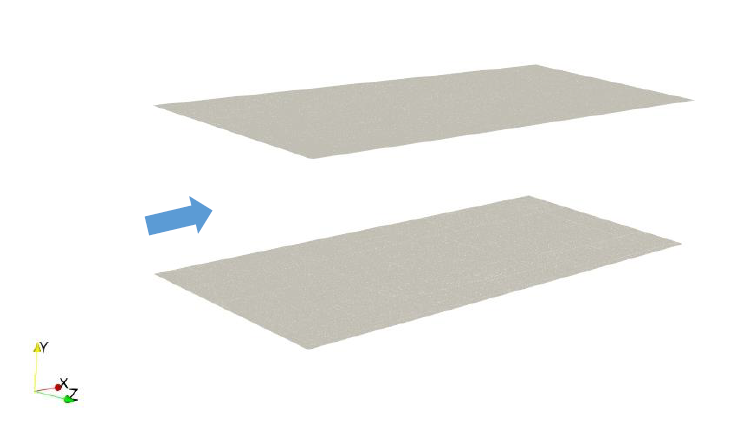
\includegraphics[width=0.9\textwidth]{figur/Infinite_plates.png}
    \caption{Flow between the infinite parallel plates}
    \label{infinite plates}
\end{figure}
%
Since the artificial periodic boundaries are enforced great care has to be taken that the domain is long enough to avoid this artificial boundary conditions from influencing the results.\emph{Moin et.al}~\cite{Moin:78} has specified certain aspects to be considered in the process of choosing the dimensions of the flow domain for the numerical simulation of the turbulent channel flow. According to~\cite{Moin:78} the experimental two-point correlation functions have to be considered for choosing the stream-wise $\left(L_x\right)$ and the span-wise $\left(L_z\right)$ lengths. The usage of periodic boundary conditions is justified if the distance between the pair of periodic boundaries is at least twice the distance, at which the correlation function becomes zero. This means that the domain size is enough to accommodate the largest eddy without the pair of periodic boundaries influencing each other.\\

To validate the LES results of the fully developed turbulent channel flow the DNS data from the database of~\cite{moser:kim:mansour:99} for the $Re_\tau = 395$ is used. The authors have shown the adequacy of the domain by performing the two-point spatial correlations. Same domain size used in~\cite{moser:kim:mansour:99} has been chosen for performing the LES of channel flow, Table \ref{Computational Domain}. Thus, no separate study for two-point correlation has been performed in this investigation.
%
\begin{table}[!h]
\centering
\begin{tabular}{c|c}
\hline
$Nominal \ret$ & $L_x$ x $L_y $x $L_z$ \\
\hline
%
395   &  $2\pi\de$ x $2\de$ x $\pi\de$  \\
\hline
\end{tabular}
\caption{The size of the domain in x, y, z directions}
\label{Computational Domain}
\end{table}\\
%
Several authors ~\cite{Freitas:11, sonja:12} have performed the turbulent channel flow simulations with smaller domain dimensions comapred to the dimensions used in the reference data, ~\cite{moser:kim:mansour:99}, in order to either save the computational time or to statiate the upper limit of the total gird points on a Graphic card~\cite{sonja:12}. But \emph{Bespalko}~\cite{bespalko:11} suggests that for performing the validation studies the dimensions of the domain should be similar to that used in the reference data. Else, the usage of smaller domain dimensions might add some kind of error and this might be than attributed to the error originating from the implementation under test.

\subsubsection{Physical parameters}
The physical parameters that are necessary for the model set-up and later on for the simulations are pressure gradient(to drive the flow), discussed in the later section, $u_\tau$, $\nu$ and $U_b$
In ~\cite{moser:kim:mansour:99} the authors have not specified $u_\tau$, $\nu$ and $U_b$ used in the simulations.~\cite{devilliers:phd} has computed and specified these parameters obtained from the DNS results of ~\cite{moser:kim:mansour:99} for $Re_\tau = 395$, Table \ref{Physical quantities}  :

%
\begin{table}[!h]
\centering
\begin{tabular}{c|c}
%\hline
$ Physical\ quantity$ & $Value\ in\ S.I\ Units$  \\
\hline
%
Half channel height, $\de$ & $1.0\ m$  \\
\hline
%
Friction velocity, $u_\tau$ & $0.0079\ m/s$  \\
\hline
%
Bulk velocity, $U_b$ & $0.1335\ m/s$  \\
\hline
%
Kinematic Viscosity, $\nu$ & $0.00002\ m^2/s$  \\
\hline
%
\end{tabular}
\caption{Physical quantities}
\label{Physical quantities}
\end{table}
%
 
In order to compute the bulk mean velocity from the DNS data (Mean stream-wise velocity), trapezoidal rule can be used to solve the equation of $U_b$ numerically. i.e. \emph{trapz} command in Matlab. 
\subsubsection{Meshing}
In order to see the effects of mesh resolution a hierarchy of meshes was created. Three uniformly spaced meshes, in all directions, were generated namely: Mesh 1 (coarse), Mesh 1\_5 (medium) and Mesh 2 (fine). The resolution of Mesh 1 was refined by a factor of 1.5 in all directions for Mesh 1\_5 and similarly by a factor of 2 for Mesh 2. To compute the mesh spacing the dimensionless distances in wall normal and wall parallel directions (stream-wise and span-wise) were used. The $u_\tau$ used for spacing computation is taken from the DNS data. Initially the plan was to go for Mesh 3, refinement by factor 4 in all directions, but the total number of mesh points were $\sim 88\ million$ ,so the idea was dropped and an intermediate mesh resolution was chosen and hence the name Mesh 1\_5.
\begin{equation}
\label{Dimensionless distances}
\begin{split}
x^+ = \frac{\Delta x u\tau}{\nu}\\
y^+ = \frac{\Delta y u\tau}{\nu}\\
z^+ = \frac{\Delta z u\tau}{\nu}\\
\end{split}
\end{equation} 
Because of the uniform meshes the spacing is same in all three directions and from now onward it will be referred as $\Delta^+$. The bottom and top faces of the domain were defined as the wall, no-slip boundary condition. The no-slip boundary condition was realized by using the half-way bounce back boundary condition. Because of the half-way bounce back boundary condition the distance of the nearest cell to the wall, $y^+$, is halved~\cite{krueger:book}. The $y^+$ will always be a smaller than $\Delta^+$ by a factor of 2. The following table \ref{Mesh statistics} shows the mesh statistics used in the investigation, where $N_x\ , N_y\ , N_z$ denote the number of nodes in the stream-wise, wall-normal and span-wise directions. In order to facilitate the grid generator the size of domain was reduced to $6\de$ x $2\de$ x $3\de$.
%
\begin{table}[!h]
\centering
\begin{tabular}{c|c|c|c|c}
%\hline
$ $ & $N_x$ x $N_y$ x $N_z$ & $Total\ nodes$ & $\sim \Delta^+$ & $\sim y^+$ \\
\hline
%
Mesh 1 & $192$ x $64$ x $96$ & $1179648$ &$12$ & $6$ \\
\hline
%
Mesh 1\_5 & $288$ x $96$ x $144$ & $3981312$ & $8$ & $4$   \\
\hline
%
Mesh 2 & $384$ x $128$ x $192$ & $9437184$ &$6$ & $3$ \\
\hline
%
\end{tabular}
\caption{Mesh statistics}
\label{Mesh statistics}
\end{table}\\
%
The domain size has been slightly altered in this investigation and this leads to the necessity for performing the two-point correlations to prove the adequacy of the domain. \emph{Premnath et.al}~\cite{Premnath:09} suggests doing it otherwise.
%
%%%%%%%%%%%%%%%%%%%%%%%%%%%%%%%%%%%%%%%%%
%
\subsection{Initial conditions}
It is known from the theory of the internal fluid flow that there exists a hydrodynamic entry length ($L_h$), starting from the inlet (x = 0), that the fluid has to travel, in the channel, for the flow to become fully developed. This means when we integrate the flow governing equations, in time, the fluid has to travel the distance $L_h$ ($\sim{x} =10H$) in every time-step, to generate a fully developed flow, which is unnecessary considering the computational efforts and also the storage requirements. The idea is to consider only that portion of the channel which will be fully developed, turbulent and neglecting the initial part ($L_h$) of the channel. This implies that specific initial conditions for the flow to become fully developed and turbulent has to be provided.\\
%
Different approaches have been used by different authors to generate the initial condition for the incompressible, three-dimensional, turbulent channel flow simulations.\emph{Moin et.al}~\cite{Moin:78} has specified few consistency criteria for initial velocity field. \emph{Sagaut}~\cite{sagaut:02} \& \emph{Fröhlich}~\cite{froehlich:book} have a concide description of most commonly used approaches with their respective advantage, disadvantages and their applications to suitable flows. Two of the several approaches mentioned in~\cite{sagaut:02} \& ~\cite{froehlich:book} will be discussed here.

\textbf{i. First approach:} In this approach a simulation is performed for some Reynolds number smaller than the one to be simulated. The resulting fields of this simulations are then used as the starting point for the required Reynolds number and is  simulated further in time until a steady state, where the statistics of the flow do not change with time, is achieved. This approach is termed as \emph{Precursor simulation} in several literature.

\textbf{ii. Second approach: } In this approach a laminar flow is chosen as the base flow and certain set of disturbances are applied on the base flow. The base flow super-imposed with disturbances is then integrated in time until the flow transitions to a turbulent flow. This approach is computationally intensive, as the flow takes time to become turbulent. There are several options available to impose the disturbances on to the base flow. Several authors have used this approach for the generating appropriate initial conditions. In this investigation this approach has been used.\\

For the initialisation of our simulations the approach of \emph{Eugene de Villiers}~\cite{devilliers:phd} was followed. \emph{Eugene de Villiers} introduced some sort of near wall streak cycle, where he uses the fundamentals of the turbulent structures near the walls. A parabolic flow profile is chosen as the base flow. To generate the parabolic flow profile the bulk mean velocity, $U_b = 0.1335\ m/s$, which was computed by \cite{devilliers:phd}, from the mean velocity DNS data of \cite{moser:kim:mansour:99} for $Re_\tau = 395$, is used.\\

Parabolic flow profile has been applied in the stream-wise direction, $u(y,0)$,  on all the fluid nodes in the domain. Figure \ref{para profile} shows the parabolic profile used as the base flow. A combination of sine and cosine waves have been used to break the flow symmetry and to develop the turbulence in the flow. 
%
\begin{figure}[h]
    \centering
    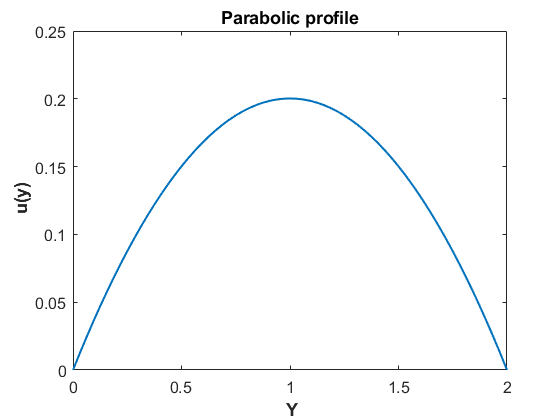
\includegraphics[width=0.6\textwidth]{figur/Parabolic_profile.png}
    \caption{Parabolic flow profile with $U_b = 0.1335\ m/s$}
    \label{para profile}
\end{figure}
%
Initially the the disturbances were applied in the stream-wise direction, but that approach was quite time consuming. It took approximately 4.5 million time-steps for the flow to become turbulent. In the next approach the disturbance was applied in the wall-normal direction, $v$. This approach reduced the time it took for the flow to becomee turbulent, ~100,000 time-steps. The exact equations for the initialization have been specified in the the eq. \ref{Initial conditions} in Appendix.

\subsection{Modelling of pressure gradient}
In the theoretical section it was shown that the pressure gradient drives the flow through a channel. With the periodic boundary conditions applied in the both streamwise and spanwise direction no information on the pressure gradient is available and thus some kind of external forcing is required to drive the flow through the channel. This requires an additional step, to model the pressure gradient, in the numerical simulation. An additional force term will be added on the right hand side of the Navier-stokes equation. Forcing is only applied in the streamwise direction, $F_x$. Two most commonly used modelling strategies will be discussed here.

\textbf{i. Constant Pressure gradient :}\\ In this approach we set $F_x$ to some constant value, thus explicitly setting the driving force, which becomes constant and uniform. 
Since the forcing is constant the mass flow rate will be varying in time, which is attributed to the wall shear stress, until the flow is fully developed (see eq. \ref{Solution equations}).
%
\begin{equation}
\label{CPG}
F_x = -\frac{\D P}{\D x} = \frac{\tau_w}{\delta} = \frac{\rho u_\tau^2}{\de}
\end{equation}
%
Thus the simulation a posteriori yields the mean flow rate, $U_b$, required to generate the prescribed frictional losses ~\cite{Quadrioa:15}. ~\cite{KPremnath:09, Freitas:11} have used this forcing strategy.

\textbf{ii. Constant Flow rate :} In this approach the forcing is not constant, but it is time dependent. The forcing is adjusted in every time step to keep the mass flow rate in the channel equal to the specified flow rate. Flow rate per channel cross-sectional area is $U_b$. Thus $U_b$ is provided as the input and we get the mean friction velocity, $u_\tau$ as the output which we compare with that of the DNS result. This is the most widely used approach in the turbulent channel simulations~\cite{devilliers:phd, sonja:12, roos:book} and it has been utilised in this investigation. Detailed description of this approach is specified rarely and the authors~\cite{Quadrioa:15, Lenormanda:00} describe the approach in detail. ~\cite{Quadrioa:15} has shown a comparison between different forcing strategies applied on the turbulent channel flow.

\subsection{Solver settings} \label{Mach reference}
Once the flow in the channel becomes turbulent, the flow is allowed to further develop in time until the it reaches a statistically steady state i.e. the statistics of the flow variables are invariant to temporal changes. Once the velocity field reaches the statistically steady state, the equations are further integrated in time to obtain the time average of the various statistical correlations and these time averaged quantities are further averaged in space along the two homogeneous directions i.e spatial averaging over the x-z planes. 

To determine the statistically steady state in the channel one can observe the evolution of the several quantities viz. turbulent kinetic energy (volume averaged), $\tau_w$, $u_\tau$ etc. over some non-dimensional time. Refer to ~\cite{Jimandmoin:91} for the detailed description for steady state determination and spatial averaging. Here two non-dimensional time will be specified \emph{large-eddy turn-over-time (LETOT)}, $tu_\tau/\de$, and the flow through the domain time, $tU_b/\de$. The $u_\tau$ obtained from DNS data is used for computing the LETOT. LETOT is the time required by the large eddy to breakdown and transfer the energy to the small eddies~\cite{bespalko:11}. In this investigation no specific quantity had been monitored to determine the statistically steady state. An estimation that $\sim10\ LETOT$ is sufficient for the flow to be fully developed and statistically steady~\cite{mk} had been followed. 

The lb simulations are generally performed in \emph{lattice units}, where all the physical parameters are represented by dimensionless numbers. This implies that converting the dimensional quantities into dimensionless lattice quantities and vice versa to interpret the simulation results. Exploiting the law of similarity we can ensure that we simulate the same kind of flow in both the unit systems by maintaining certain non-dimensional parameters equal in both unit systems i.e. Reynolds number.
 
LB is mostly used for simulating the incompressible fluids where the Mach number is smaller $\left(Ma<0.3\right)$. The flow in this investigation is also incompressible. Smaller Mach number $Ma\ll 1$ implies that the flow in the channel evolves with smaller time-step, $\Delta t$, i.e. flow evolves slowly and thus renders the simulation as computationally expensive. In order to avoid that, $Ma$ has been artificially increased to speed-up the simulation i.e. coarser $\Delta t$ by keeping the $Re$ number constant. The computation of the parameters required to increase the $Ma$ is specified in the Appendix.  The table  \ref{Mach settings} shows the actual, $Ma_{act}$, and the artificial, $Ma_{art}$, Mach number.\\
%
\begin{table}[h!]
\begin{center}
\begin{tabular}{ p{2.2cm}|p{2cm} } 
\hline
Mach number & Value \\
  \hline
  \multirow{1}{5em}{$Ma_{act}$} & 0.000389213 \\
  \hline
  \multirow{1}{5em}{$Ma_{art}$} & 0.180647487 \\
  \hline
\end{tabular}
\end{center}
\caption{Mach number}
\label{Mach settings}
\end{table}
%
\\
There are two stages in the simulation of turbulent channel flow: Flow development stage and the averaging stage. In the flow development stage the flow is allowed to develop till it reaches the statistically steady state and in the averaging stage the statistics of the flow variables are sampled. Table \ref{Solver settings} shows the time, dimensional and non-dimensional values, required by different mesh resolutions for each stage.
%
\begin{table}[h!]
\begin{center}
\begin{tabular}{ |p{2cm}|p{1.5cm}|p{2cm}|p{2cm}|p{2cm}|  } 
\hline
 &$\sim time$ & Mesh1 & Mesh1\_5 & Mesh2 \\
  \hline
  \multirow{3}{6em}{Flow developing stage} & $t\ [s]$ & 7324 & 9806 & 12871\\
  & $tu_\tau/\delta$ & 57 & 77 & 101\\ 
  & $tU_b/\delta$ & 977 & 1309 & 1718\\ 
  \hline
  \multirow{3}{6em}{Averaging stage} & $t [s]$ & 65917 & 76002 & 69873\\
  & $tu_\tau/\delta$ & 520  & 600 & 552\\ 
  & $tU_b/\delta$ & 8800 & 10146 & 9328\\ 
  \hline
\end{tabular}
\end{center}
\caption{Solver settings}
\label{Solver settings}
\end{table}
%
As suggested by~\cite{mk} $\sim10\ LETOT$ is sufficient for the flow development stage, but the table \ref{Solver settings} shows some higher values as it also involves the duration over which the flow becomes turbulent.
In the averaging stage the averaging was carried out for longer duration to make sure that we have symmetric Reynolds stress component profiles. This decision was made after observing the profiles generated from every temporal and spatial averaged data set. Mean velocity profiles relatively require less time to have a steady symmetric profile.
%%
%\begin{table}[h!]
%\begin{center}
%\begin{tabular}{|r||r@{--}l|p{4cm}|}
%\hline
%\multicolumn{4}{|c|}{Eine aufwendige Tabelle} \\ \hline \hline
%& \multicolumn{2}{c|}{Flow developing stage} & \\ \cline{2-3}
%\multicolumn{1}{|c||}{J.}
%& \multicolumn{1}{r@{\,\vline\,}}{niedrig} & hoch &
%\multicolumn{1}{c|}{Averaging stage} \\ \hline
%2012 & 25 & 370 & Schlechtes Jahr. \\ \hline
%13 & 350 & 390 & Stabile Preise. Es geht aufwärts. \\ \hline
%\end{tabular}
%\end{center}
%\caption{Solver}
%\end{table}

\subsection{Computational details \& Post-processing}
Simulations have been carried out on the Phoenix cluster~\cite{phoenix} of TU Braunschweig. Computations have been performed on the one of the 8 available GPU nodes. Visualisation of the large data sets has been performed using the one of the 6 available visualisation nodes on the cluster.
Time averaging of the flow variables along with the other turbulence statistics is performed during the simulations within the solver itself i.e. running time average as referred in the literature~\cite{Moin:78}. Spatial averaging is performed a posteriori in Matlab. Paraview together with python scripting is used to manipulate and extract the data from the resulting time-averaged data sets. Paraview is also used for the visualisation of the instantaneous data i.e. velocity contour plots, iso-volumes etc. The data extracted by the python scripts is then used by the Matlab scripts to further manipulate and visualise the data in the form of profile plots i.e mean velocity profiles, Reynolds stresses.



 


\newpage
%\chapter{Results and discussion}

\section{Results and discussion}
In this section the results of the simulations will be presented and discussed. Two different variations of the LB solver were tested. One with the optimised values of the relaxation parameters~\cite{geier:parameter} and other with the relaxation parameters used as specified in ~\cite{geier:cumulant}. The results presented in this section are performed with the former variation of the LB solver  and the results of the latter variation will just be presented in the Appendix, as the choice of value one for all the parameters is the most stable choice but not accurate enough~\cite{geier:parameter}. Firstly, the results of the LB simulations carried out without any turbulence model will be presented and discussed. The result of the simulations with no-model will be termed as the \emph{under resolved DNS} (UDNS). Under resolved because the resolution is coarser compared to the reference mesh resolution and DNS because no additional modelling is done for turbulence. It will be followed by the discussion of the results from the LB-LES with the WALE model and will be compared with the UDNS and DNS results. Few general comments applicable for all the simulations are:

\begin{itemize}
\item The DNS results of~\cite{kim:moin:moser:87} , for $Re_\tau = 395$, will be used as a reference for the comparison. The quantities obtained from the DNS data will be referred to as the \emph{target} quantities.
\item The results shown here are plotted against the global coordinates, $y/\de$, and local coordinates,  $y^+$.  
\item All simulations have been performed using the single precision on GPGPUs. 
\item The normalised wall distance $y^+$ used in the profile plots is computed a posteriori for all the simulations.
%\item Since the channel flow is symmetric, the profiles have been plotted over the  
\end{itemize}

\subsection{UDNS results} \label{UDNS profiles}
To test the accuracy of the turbulent channel flow results from the LB solver, against the DNS data, these simulations have been performed. The physical quantities resulting from the simulations for all meshes are listed in the table (\ref{Global quantities}). The average friction velocity ($u_\tau$) and the $Re_\tau$ resulting from the computed $u_\tau$ are the important quantities. From now on $u_\tau$ represents the average friction velocity. The computed value of $u_\tau$ is under-predicted for all the simulations and so is the resulting $Re_\tau$, but the values approach the target $u_\tau$ with the increase in the mesh resolution. We know from the definition of $u_\tau$,that $u_\tau$ is proportional to the $\tau_w$. Thus, smaller values of the $u_\tau$ implies smaller values of $\tau_w$.  
%
\begin{table}[h!]
\begin{center}
\begin{tabular}{ p{3cm}|p{1.5cm}p{1.5cm}p{1.5cm}p{1.5cm}  } 
\hline
Physical quantity & Mesh1 & Mesh1\_5 & Mesh2 & Target \\
  \hline
  \multirow{1}{6em}{$u_\tau,\ m/s$}  & 0.0070 & 0.0074 & 0.0076 & 0.0079\\
  \hline
  \multirow{1}{6em}{$Re_\tau$} & 352 & 371 & 382 & 395\\
  \hline
  \multirow{1}{6em}{$U_c,\ m/s$} & 0.1565 & 0.1563 & 0.1557 & 0.1591\\
  \hline
\end{tabular}
\end{center}
\caption{Comparison of the resulting physical quantities}
\label{Global quantities}
\end{table}
%
\subsubsection{Mean velocity profile} \label{Mean velocity UDNS}

Mean velocity profiles presented here have been averaged in time and space. It is seen from the Fig. (\ref{Mean velocity global}) and Fig. (\ref{Mean velocity wall}), the mean velocity profiles for all the meshes over-predict the DNS data. As discussed in the section \ref{scaling} the viscous sublayer plays a dominant role on the flow characteristics as higher velocity gradients are present there. Since the viscous sublayer is under-resolved in the simulations, $u_\tau$ and eventually the $\tau_w$ is under-predicted and as a result we see the different flow characteristics obtained from the simulations i.e. over-predicting velocity profiles in comparison to the DNS data. It is clear that with the better resolution of the viscous sublayer, the correct flow characteristics will be obtained and it is apparent from the Fig. (\ref{Mean velocity global}) and Fig. (\ref{Mean velocity wall}) that with the mesh refinement, the velocity profiles approach closer to the DNS data. Velocity profile for mesh3 nearly collapses on to the DNS data. Thus a positive effect of mesh resolution is seen from the mean velocity profile plots. 
%
\begin{figure}[h]
    \centering
    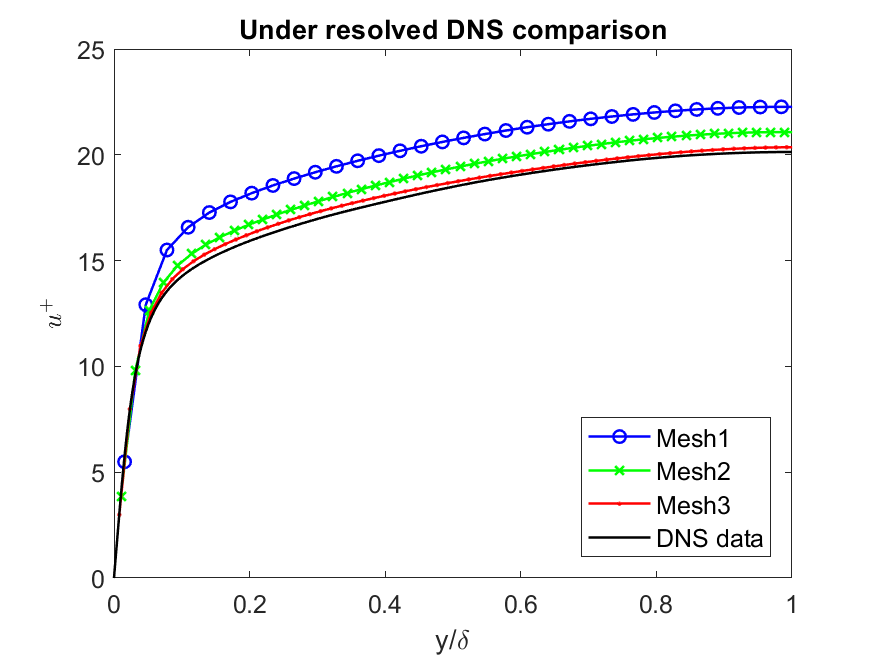
\includegraphics[width=0.95\textwidth]{06_Resultsanddiscussion/figur/UDNS_2016/Profile_global_coords.png}
    \caption{Mean stream-wise velocity profile normalized by $u_\tau$, plotted in global coordinates}
    \label{Mean velocity global}
\end{figure}

\begin{figure}[t]
    \centering
    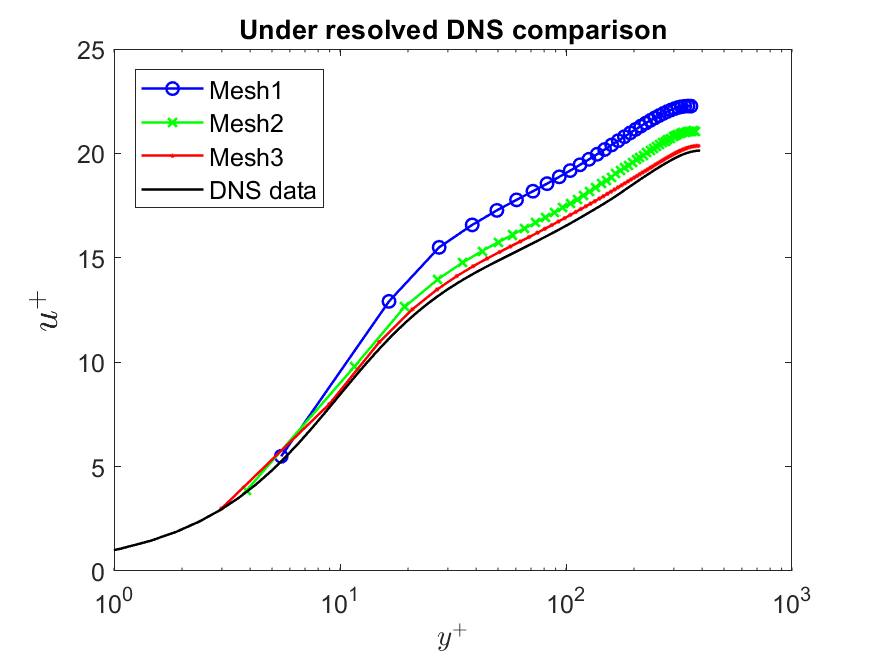
\includegraphics[width=0.95\textwidth]{06_Resultsanddiscussion/figur/UDNS_2016/Profile_wall_coords_theo_comp.png}
    \caption{Mean stream-wise  velocity profile normalized by $u_\tau$, plotted in wall coordinates (semi-log plot)}
    \label{Mean velocity wall}
\end{figure}

\subsubsection{Turbulence intensities} \label{Turbulence intensities UDNS}
Turbulence intensities is the term used for the root-mean-square (rms) profiles of the velocity fluctuations. The rms profiles shown in this section have been averaged in the following order: 
the time-averaged data set written out in every time-step is spatially averaged and these time and space averaged data sets are again time-averaged to have symmetric rms profiles. The Fig. \ref{Turbulence intensities} shows the rms velocity fluctuations plotted in the global coordinates. The rms profiles are symmetric about the half-channel height i.e. $y = \de$ and the symmetry of the profiles about $\de$ indicates the adequacy of the sampling taken for average ~\cite{kim:moin:moser:87}. Turbulence intensities normalised by $u_\tau$ are compared with different mesh resolutions and the DNS data\footnote{the DNS data for the velocity fluctuation profiles have been provided as variances ($\overline{{\up}^2}$) and not the rms ($\sqrt{\overline{{\up}^2}}$)values}. 
%
\begin{figure}[h!]
    \centering
    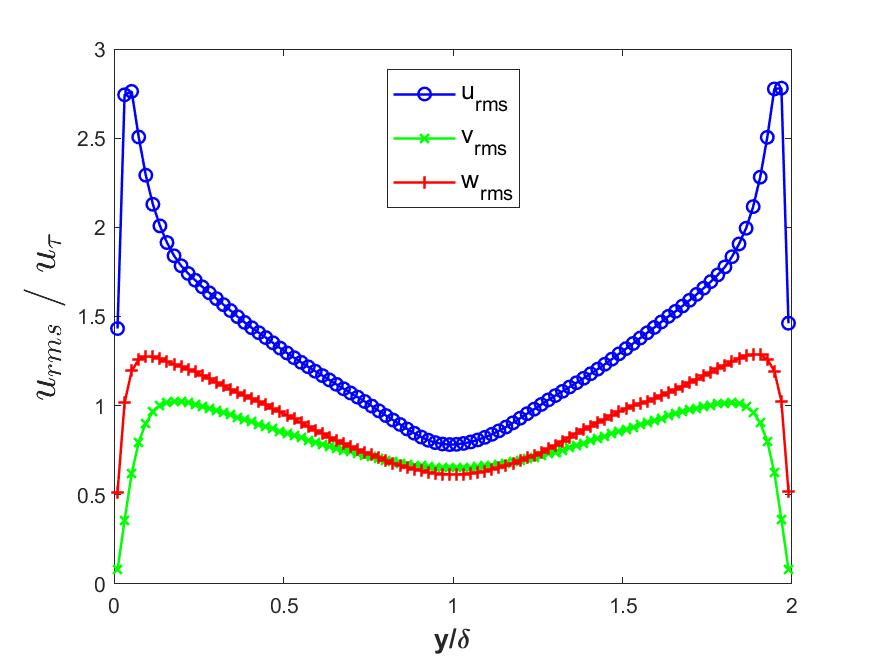
\includegraphics[width=0.6\textwidth]{06_Resultsanddiscussion/figur/UDNS_2016/Turbulence ontensities_Mesh2.jpg}
    \caption{Root-mean-square velocity fluctuations normalized by $u_\tau$ in global coordinates}
    \label{Turbulence intensities}
\end{figure}
%

Fig.(\ref{urms wall})-(\ref{wrms wall}) shows the comparison of the components of the rms profiles of the streamwise, wall-normal and spanwise velocity fluctuations, respectively, with the different mesh resolutions and the DNS data in wall coordinates. The profiles do not start from zero value, as only the fluid nodes are plotted. The general observation from all three velocity fluctuation profiles is that they converge to the DNS data with the increase in the mesh resolution. 

Mesh 2 and Mesh 3 accurately estimates the location of the peak values for all three velocity component profiles, respectively, compared to the DNS data. Mesh 3 for all the velocity component profiles predict the peak value fairly close to that of the DNS data. All three velocity component profiles for Mesh 3 are in fairly good agreement with the DNS data. 

The rms value of the streamwise profile increases from zero at the wall to some peak value in either buffer layer, $5<y^+< 30$, or in the log-law layer, $y^+ > 30\  till\  y/\de <0.3$ and then drops gradually towards the centre of the channel. The velocity profile for the wall-normal component develops slowly in comparison to the streamwise and the spanwise component profiles. The approximate location of the peak value for streamwise profile (DNS) is at $y^+ = 14$ \cite{kim:moin:moser:87} i.e. buffer layer. The location of peak value for the spanwise component (DNS) is at $y^+ = 40$ i.e. log-law region and the location for the wall-normal component (DNS)is at $y^+ = 70$ also in the log-law region, but towards the end of it. The resulting profiles of Mesh 3 for all components approximately shows the same locations for the peak values as that of the corresponding DNS data.
%%
%\begin{table}[h!]
%\begin{center}
%\begin{tabular}{ p{1cm}|p{1.5cm}p{1.5cm}p{1.5cm}p{1.5cm}  } 
%\hline
% & Mesh1 & Mesh2 & Mesh3 & DNS \\
%  \hline
%  \multirow{1}{6em}{$y^+$} & 17 & 15 & 14.93 & 14\\
%  \hline
%\end{tabular}
%\end{center}
%\caption{Peak values of the rms profiles of stream-wise velocity fluctuations}
%\label{Peak values}
%\end{table}
%%
%
\begin{figure}[h]
%\centering
\begin{minipage}[b]{0.5\textwidth}
\subfigure[Zoom near the wall]{
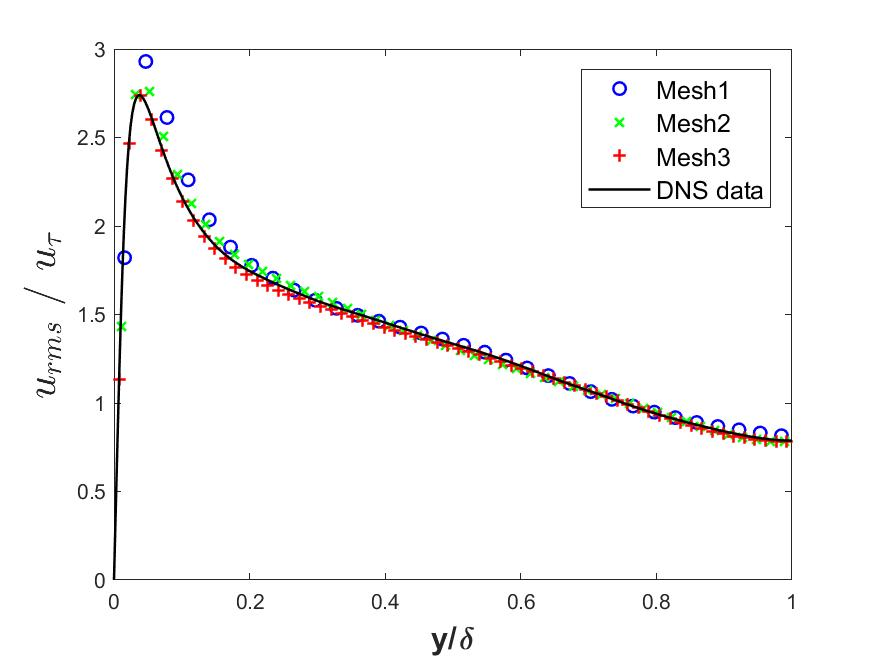
\includegraphics[width=6.7cm]{06_Resultsanddiscussion/figur/UDNS_2016/urms_global_coords.jpg}}
\end{minipage}
%
\begin{minipage}[b]{0.5\textwidth}
\subfigure[Outer region]{
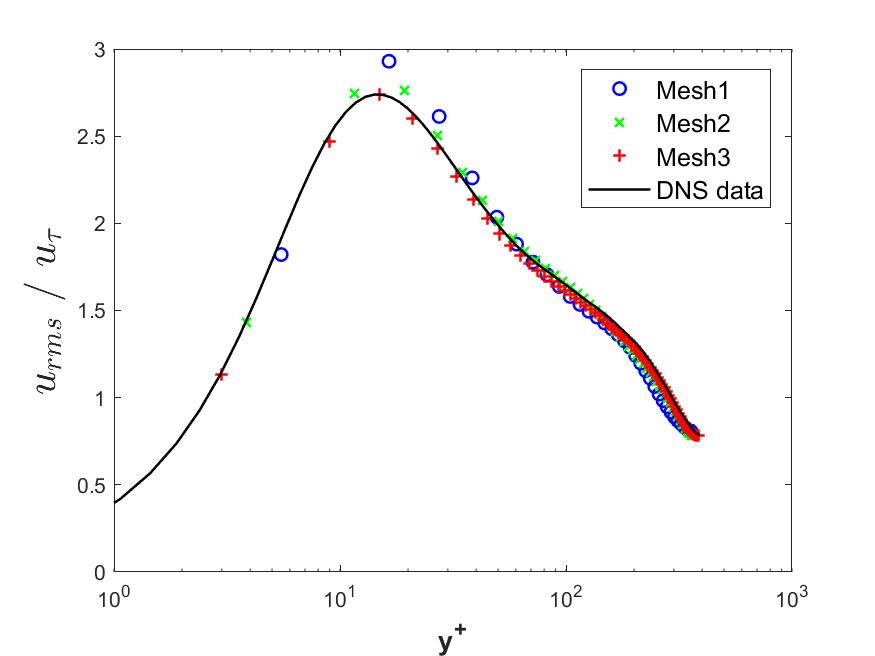
\includegraphics[width=6.7cm]{06_Resultsanddiscussion/figur/UDNS_2016/urms_wall_coords.jpg}}
\end{minipage}
\caption{Channel flow at $Re_\tau=2000$}
\label{uv_balance}
\end{figure}


\begin{figure}[h!]
    \centering
    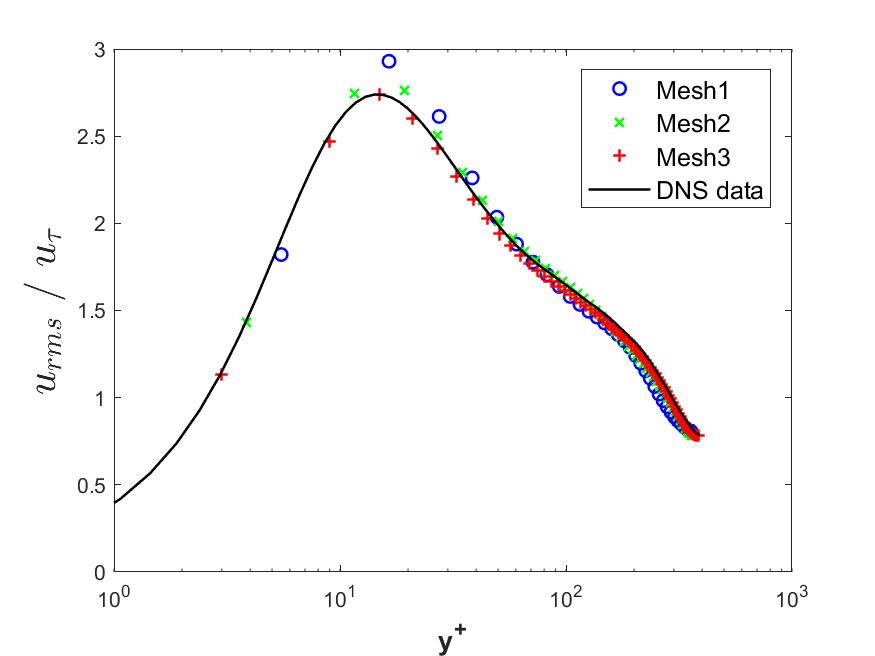
\includegraphics[width=0.6\textwidth]{06_Resultsanddiscussion/figur/UDNS_2016/urms_wall_coords.jpg}
    \caption{$u_{rms}$ normalized by $u_\tau$ in wall coordinates}
    \label{urms wall}
\end{figure}

\begin{figure}[h!]
    \centering
    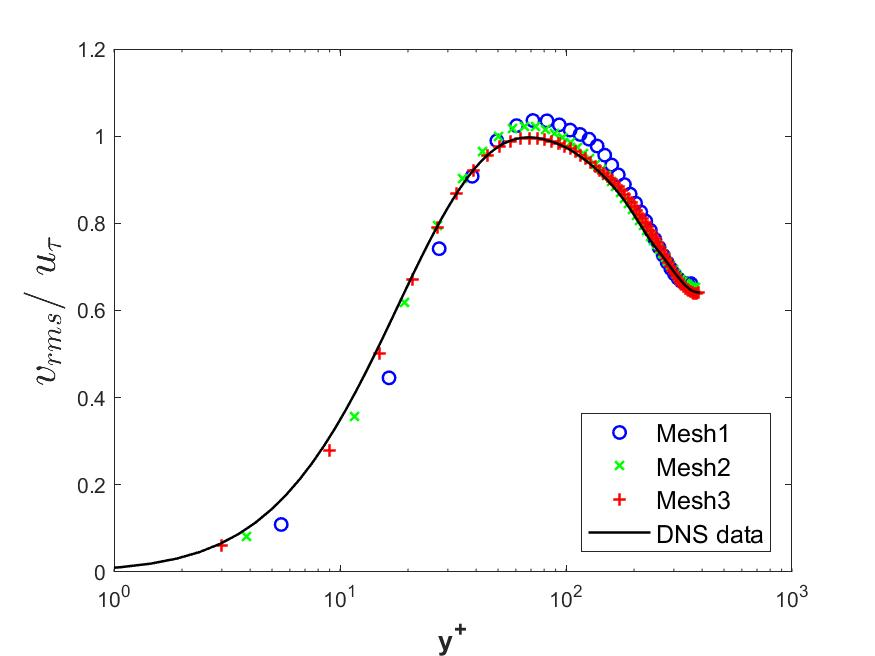
\includegraphics[width=0.6\textwidth]{06_Resultsanddiscussion/figur/UDNS_2016/vrms_wall_coords.jpg}
    \caption{$v_{rms}$ normalized by $u_\tau$ in wall coordinates}
    \label{vrms wall}
\end{figure}

\begin{figure}[h!]
    \centering
    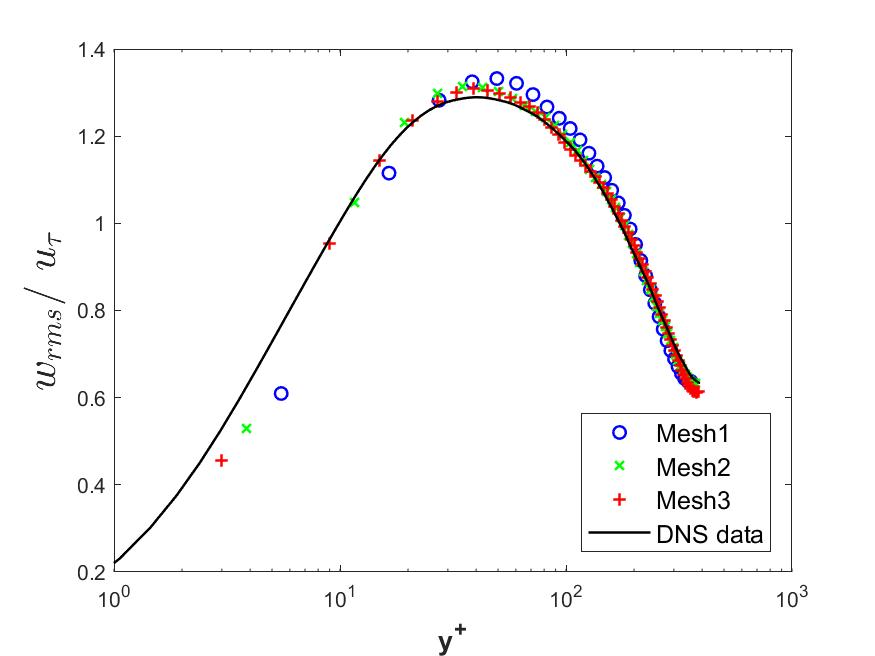
\includegraphics[width=0.6\textwidth]{06_Resultsanddiscussion/figur/UDNS_2016/wrms_wall_coords.jpg}
    \caption{$w_{rms}$ normalized by $u_\tau$ in wall coordinates}
    \label{wrms wall}
\end{figure}

\subsubsection{Turbulent shear stress}
Turbulent shear stress is also referred to as the co-variance of the Reynolds stress tensor i.e. $-\overline{\up\vp}$. This component is responsible for the turbulent diffusion of the momentum. It is also sometimes referred to as the resolved shear stress. 

Fig. (\ref{uvrms wall}) shows the turbulent shear stress profile normalised with the $u_\tau^2$ plotted in wall coordinates and compared against the DNS data and with the mesh resolutions.
\begin{figure}[h!]
    \centering
    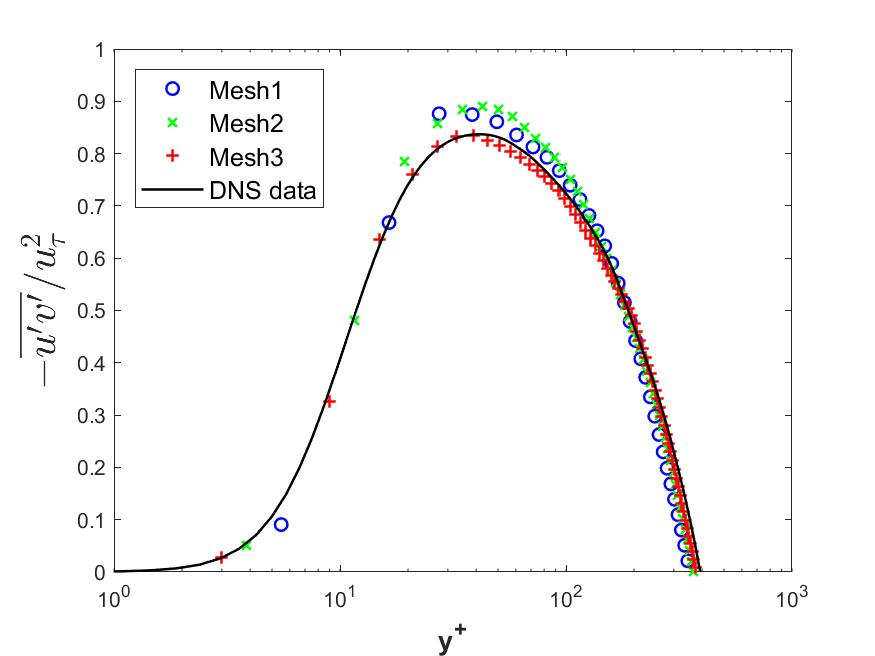
\includegraphics[width=0.6\textwidth]{06_Resultsanddiscussion/figur/UDNS_2016/uv_rms_wall_coords.jpg}
    \caption{$uv_{rms}$ normalized by $u_\tau$ in wall coordinates}
    \label{uvrms wall}
\end{figure}

As seen from the Fig. (\ref{uvrms wall}) the increase in the mesh resolution results in the better agreement to the DNS data. Mesh 3 here shows a very good agreement to the DNS data and also it predicts the location of the peak value, $y^+ = 35$ fairly well.
\subsection{WALE model results}
In this section the results obtained from the combination of the LB flow solver with the WALE model (LES) performed on the relatively coarser mesh, in comparison to the resolution of the DNS data, will be presented. The main purpose is to access the accuracy with which the aforementioned combination reproduces the mean flow profiles and other turbulence statistics when compared to the DNS data. The computed physical quantities have been listed in the table \ref{Global quantities WALE} for all mesh resolutions. The same trend is seen for the physical quantities as mentioned in the section \ref{UDNS profiles}. The physical quantities approach closer to the respective target values with the increase in the mesh resolution. 
%
\begin{table}[h!]
\begin{center}
\begin{tabular}{ p{3cm}|p{1.5cm}p{1.5cm}p{1.5cm}p{1.5cm}  } 
\hline
Physical quantity & Mesh1 & Mesh2 & Mesh3 & Target \\
  \hline
  \multirow{1}{6em}{$u_\tau,\ m/s$}  & 0.0069 & 0.0073 & 0.0075 & 0.0079\\
  \hline
  \multirow{1}{6em}{$Re_\tau$} & 347 & 367 & 377 & 395\\
  \hline
  \multirow{1}{6em}{$U_c,\ m/s$} & 0.1562 & 0.1557 & 0.1547 & 0.1591\\
  \hline
\end{tabular}
\end{center}
\caption{Comparison of the computed physical quantities using WALE model}
\label{Global quantities WALE}
\end{table}
%
\subsubsection{Mean velocity profiles}
The mean velocity profiles, normalised with the $u_\tau$, presented here are averaged in time and space. Fig. (\ref{Mean profiles WALE}(a-b)) shows the mean velocity profiles plotted in the global and local coordinates. It is clear from the both the figures that with increase in the mesh resolution the velocity profiles approach closer to the DNS data. All profiles over-predict the DNS data, but the velocity profile for the mesh 3 is relatively in good agreement with the DNS data. The reason for the over-prediction is similar to that explained in section \ref{Mean velocity UDNS}.
%%% Mean veloity profiles %%%
\begin{figure}[h!]
%\centering
\begin{minipage}[b]{0.5\textwidth}
\subfigure[global coordinates]{
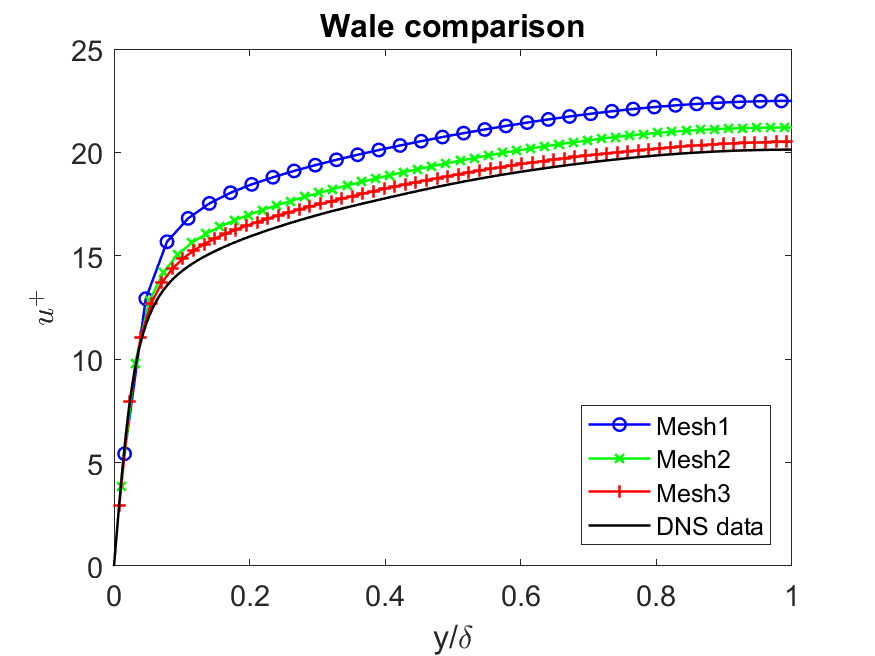
\includegraphics[width=6.7cm]{06_Resultsanddiscussion/figur/WALE/Profile_global_coords.png}}
\end{minipage}
%
\begin{minipage}[b]{0.5\textwidth}
\subfigure[wall coordinates]{
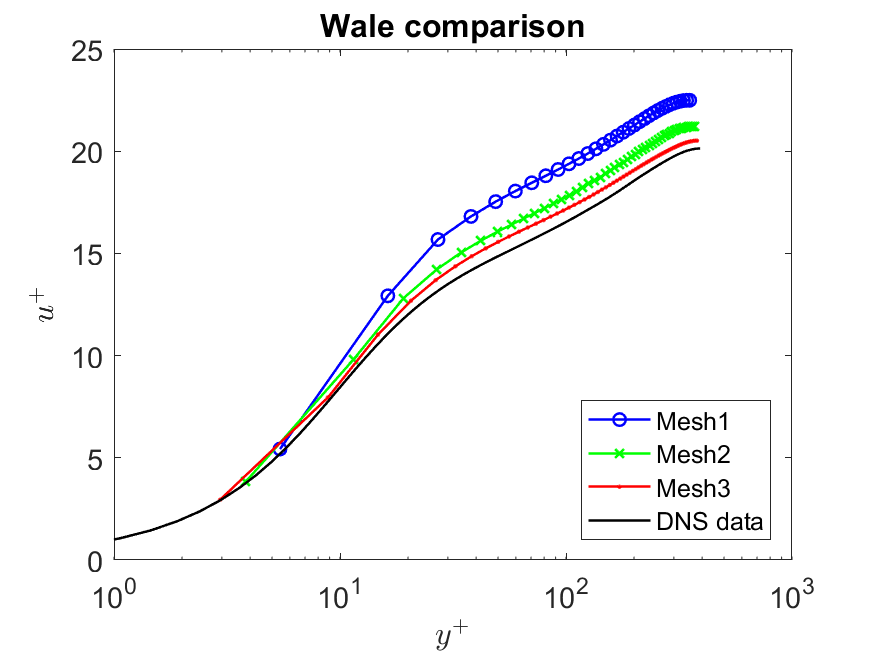
\includegraphics[width=6.7cm]{06_Resultsanddiscussion/figur/WALE/Profile_wall_coords_theo_comp.png}}
\end{minipage}
\caption{Mean velocity profile normalised with $u_\tau$}
\label{Mean profiles WALE}
\end{figure}
%%% End mean velociy profiles %%%%
\subsubsection{Turbulence intensities}
The rms profiles presented here are averaged in the same fashion as that of the section \ref{Turbulence intensities UDNS}. To show the adequacy of sampling taken for averaging the symmetric rms profiles, about the half-channel height $y  = \de$, of all three velocity fluctuations is shown in Fig. (\ref{Turbulence intensities WALE}). The comments made in the section \ref{Turbulence intensities UDNS} for the velocity profiles are also applicable here.
%
\begin{figure}[h!]
    \centering
    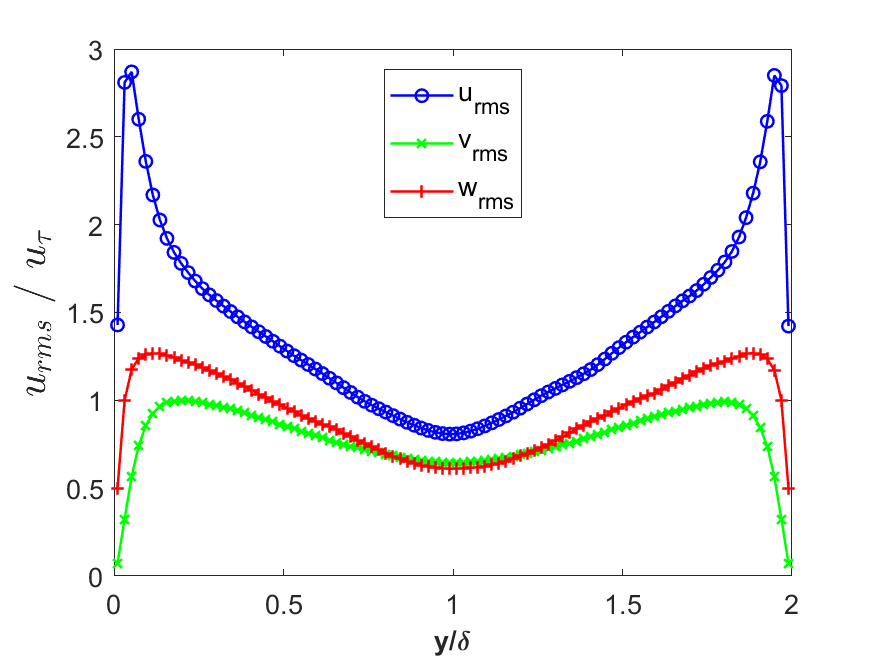
\includegraphics[width=0.6\textwidth]{06_Resultsanddiscussion/figur/WALE/Turbulence intensities_Mesh2.png}
    \caption{Root-mean-square velocity fluctuations normalized by $u_\tau$ in global coordinates}
    \label{Turbulence intensities WALE}
\end{figure}
%
The rms velocity profiles for all three components show a good agreement towards the DNS data as the mesh resolution increases. 
%
\begin{figure}[h!]
%\centering
\begin{minipage}[b]{0.5\textwidth}
\subfigure[global coordinates]{
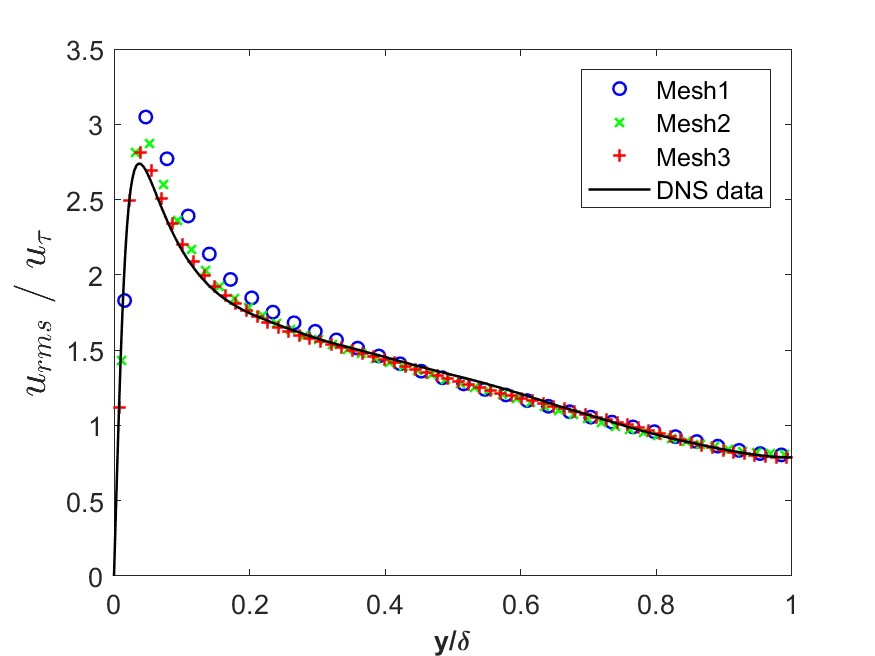
\includegraphics[width=6.7cm]{06_Resultsanddiscussion/figur/WALE/urms_global_coords.png}}
\end{minipage}
%
\begin{minipage}[b]{0.5\textwidth}
\subfigure[local coordinates]{
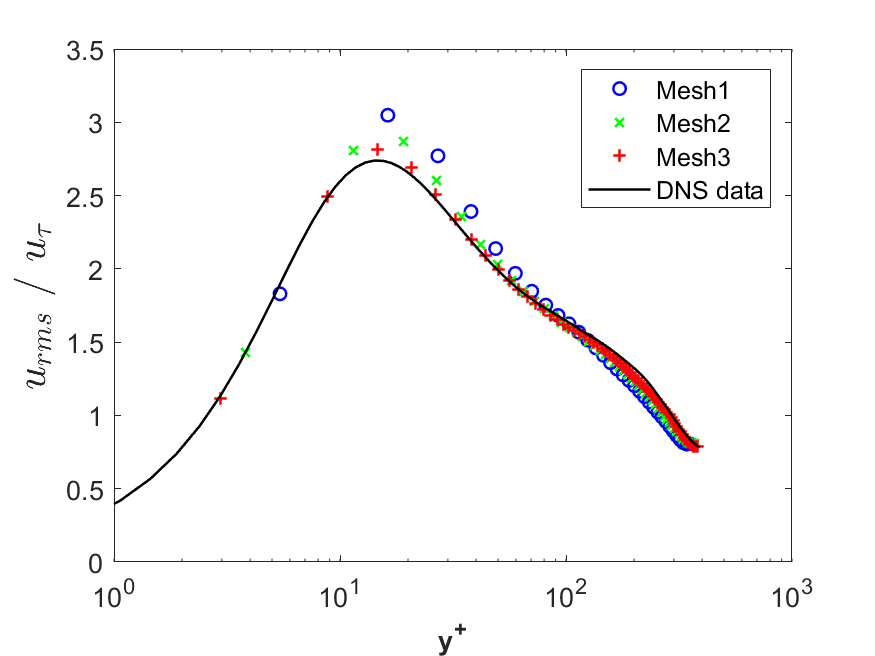
\includegraphics[width=6.7cm]{06_Resultsanddiscussion/figur/WALE/urms_wall_coords.png}}
\end{minipage}
\caption{Rms profiles for the streamwise velocity fluctuation normalised by $u_\tau$}
\label{urms wale}
\end{figure}
%% End %%
%
\begin{figure}[h!]
%\centering
\begin{minipage}[b]{0.5\textwidth}
\subfigure[global coordinates]{
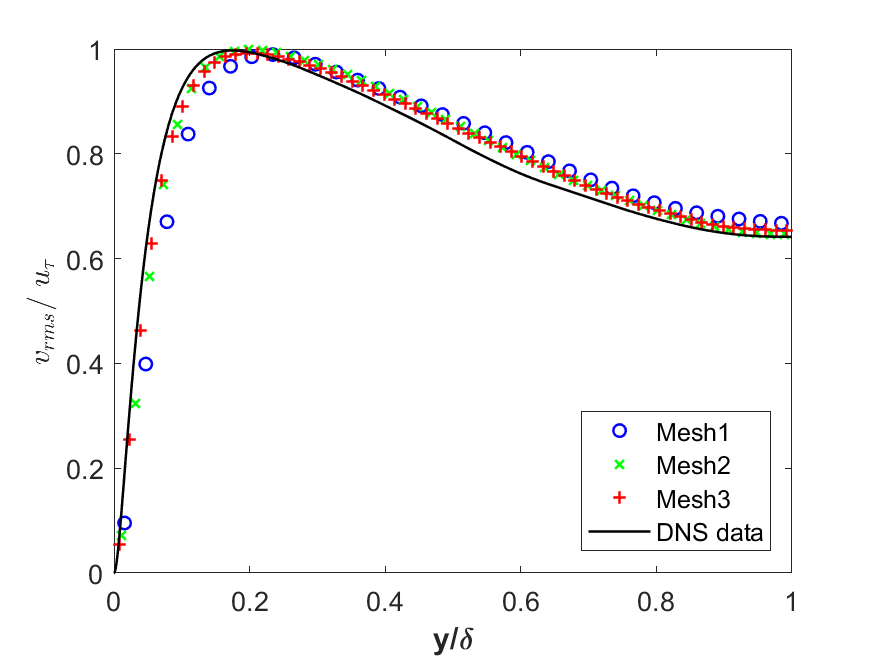
\includegraphics[width=6.7cm]{06_Resultsanddiscussion/figur/WALE/vrms_global_coords.png}}
\end{minipage}
%
\begin{minipage}[b]{0.5\textwidth}
\subfigure[local coordinates]{
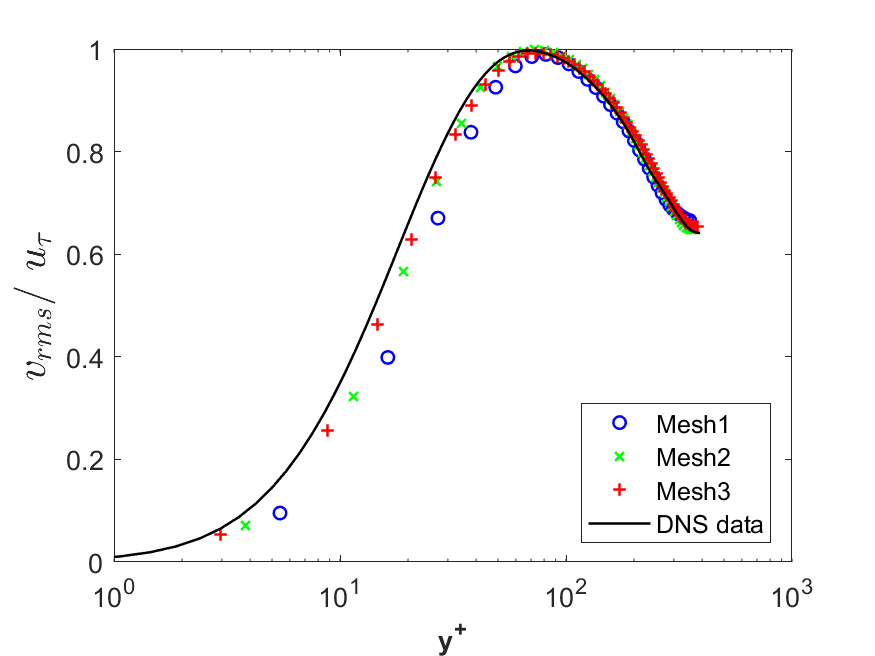
\includegraphics[width=6.7cm]{06_Resultsanddiscussion/figur/WALE/vrms_wall_coords.png}}
\end{minipage}
\caption{Rms profiles for the wall-normal velocity fluctuation normalised by $u_\tau$}
\label{vrms wale}
\end{figure}
%% End %%
%
\begin{figure}[h!]
%\centering
\begin{minipage}[b]{0.5\textwidth}
\subfigure[global coordinates]{
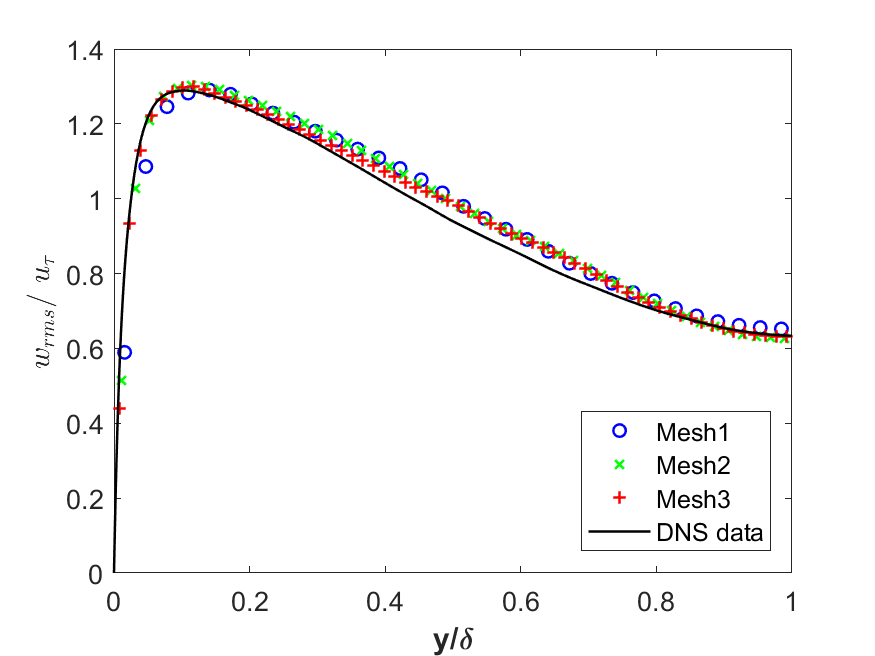
\includegraphics[width=6.7cm]{06_Resultsanddiscussion/figur/WALE/wrms_global_coords.png}}
\end{minipage}
%
\begin{minipage}[b]{0.5\textwidth}
\subfigure[local coordinates]{
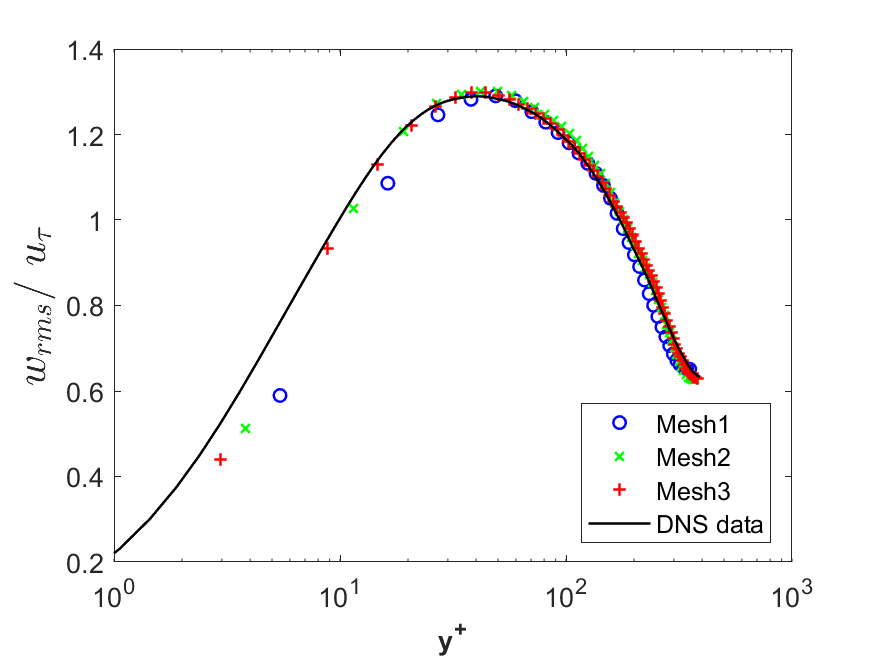
\includegraphics[width=6.7cm]{06_Resultsanddiscussion/figur/WALE/wrms_wall_coords.png}}
\end{minipage}
\caption{Rms profiles for the spanwise velocity fluctuation normalised by $u_\tau$}
\label{wrms wale}
\end{figure}
%% End %%
\subsubsection{Turbulent shear stress}
%
\begin{figure}[h!]
%\centering
\begin{minipage}[b]{0.5\textwidth}
\subfigure[global coordinates]{
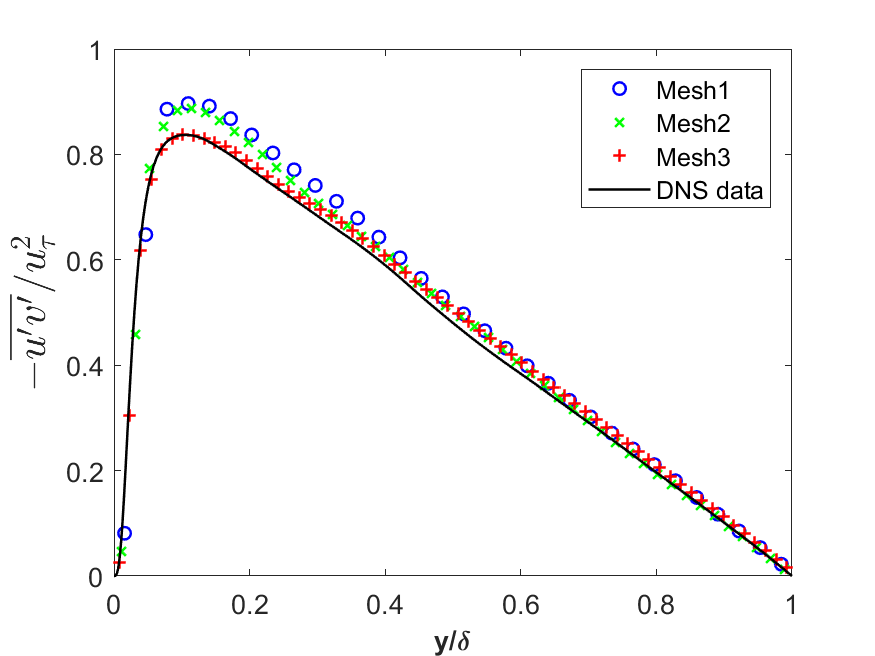
\includegraphics[width=6.7cm]{06_Resultsanddiscussion/figur/WALE/uv_rms_global_coords.png}}
\end{minipage}
%
\begin{minipage}[b]{0.5\textwidth}
\subfigure[local coordinates]{
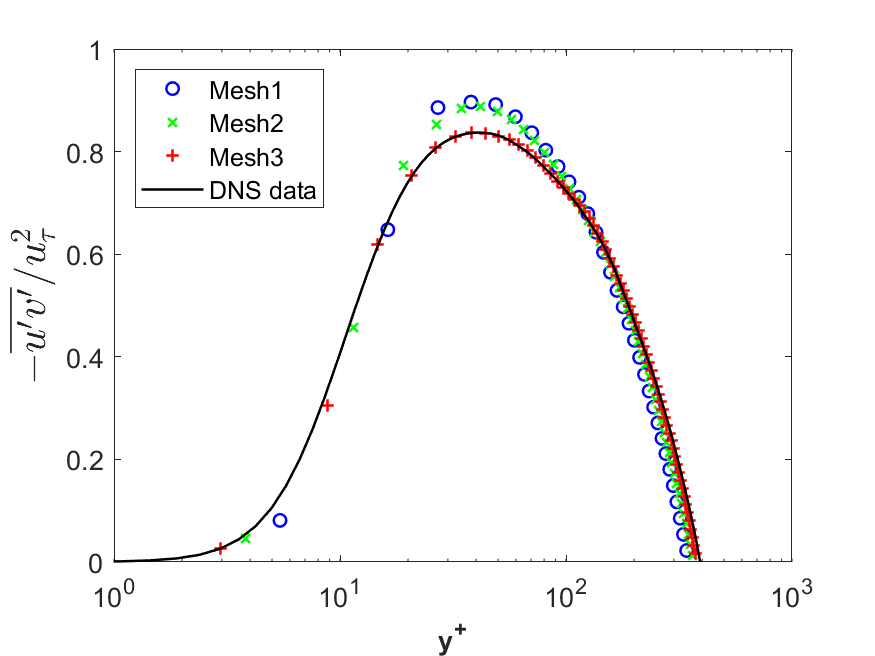
\includegraphics[width=6.7cm]{06_Resultsanddiscussion/figur/WALE/uv_rms_wall_coords.png}}
\end{minipage}
\caption{Turbulent shear stress profiles normalised by $u_\tau$}
\label{uvrms wale}
\end{figure}
%% End %%
%\subsection{Comparison UDNS and WALE}

\clearpage
\newpage

\appendix

\section{Appendices}

\subsection{Initial conditions} \label{I.C}

The following are the initial conditions, for density and the velocity components resp, used for fully developed channel flow simulations:

\begin{multline}
\rho = 27\ U_b^2 \left( cos\left(x\right) \frac{4\pi}{x} + cos\left(y\right) \frac{4\pi}{y}\right) \frac{y}{x} \\+  27\ U_b^2 \left( cos\left(x\right) \frac{4\pi}{x} + cos\left(z\right) \frac{4\pi}{z}\right) \frac{z}{x}
\end{multline}

\begin{equation}
\label{Initial conditions}
\begin{split}
u &= 3* U_b \left(\frac{y}{h} - 0.5\left(\frac{y^2}{h^2}\right)\right)\\
v &= U_b* cos\left(x\right)\frac{2\pi}{x}*sin\left(y\right)\frac{2\pi}{y} \\
w &= 0\\
\end{split}
\end{equation}\\
\label{Initial condition}


\subsection{Lattice units} \label{Mach number explanation}

As mentioned earlier the lattice units are the dimensionless lattice values of the corresponding physical parameters. Chapter 7 in~\cite{krueger:book} provides the detailed explanation on how to non-dimensionalise and several considerations while performing that to the physical units. For the further discussion the lattice units will be marked with an asterisk, *, sign and the unmarked symbols will represent the physical parameters. As mentioned earlier to simulate the same flow, the Reynolds number in both the unit systems has to be equal. Here the $Re_b$ is taken as the reference.
%
\begin{equation}
\label{Law of similarity}
\begin{split}
Re^* &= Re_b\\
\frac{ U^*l^*}{\nu^*}  &= \frac{U_b\ l}{\nu}\\
\end{split}
\end{equation}
%
The total number of grid nodes are same in both unit system, thus :
\begin{equation}
\label{Length lb}
\begin{split}
N^* &= N\\
\frac{l^*}{{\Delta x}^*}  &= \frac{l}{{\Delta x}}\\
l^*  &= \frac{l}{{\Delta x}} {\Delta x}^*\\
\end{split}
\end{equation}
The usage of the uniform grid here implies that ${\Delta x}^* = 1$. With the same assumption as of Reynolds number the lattice and the physical Mach number must also match and this implies:
\begin{equation}
\label{Length lb}
\begin{split}
Ma^* &= Ma\\
\frac{U^*}{{c_s}^*}  &= \frac{U_b}{{c_s}}\\
U^*  &= Ma\ {{c_s}^*}\\
\end{split}
\end{equation}
%
where $c_s^*$ is the lattice speed of sound and equal to $\frac{1}{\sqrt{3}}$ $\approx 0.577$. When simulating the incompressible flow simulations the Mach number is small and hence it is not necessary to equate the Mach number until and unless it is small. Mach number is lattice units is considered small when $Ma^*<0.3$~\cite{krueger:book}.
Now $l^*$ and $U^*$ are known the only free parameter $\nu^*$ can be computed by using the eq. \ref{Law of similarity}.

As mentioned before the Mach number of the simulation is very small i.e. $Ma\ll 1$, as the flow is incompressible. This means that the $U^*$ will be very small and thus $\Delta t$ which scales as $\Delta t \propto Ma^*$ will also be very small. The total simulation time, T, is expressed as ~\cite{krueger:book} $$ T \propto \frac{1}{\Delta x^n \Delta t}$$
where n is the spatial dimension. This shows that smaller $\Delta t$ requires a large number of time-steps for the flow to develop. Hence it is suggested to some how increase $Ma^*$ and eventually $U^*$ as $U^* \propto Ma^*$.
Let us consider an example of Mesh 1 resolution to show how the Mach number was increased. 
\begin{equation}
\label{Art Ma}
\begin{split}
U^* &= \frac{Re_b \nu^*}{l^*}\\
Ma^* &= {U^*}{\sqrt{3}}\\
\end{split}
\end{equation}
%
$l^* = 64$ and $\nu^*$ is chosen equal to 0.0005 and the resulting $U^* = 0.104296875
$. With the increase in the mesh resolution the $\nu^*$ also increases to keep the Reynolds number same. Thus the eq. \ref{Art Ma} show how the $Ma^*$ has been increased. The intrinsic restrictions of LB algorithm however puts a limit on the simulation parameters i.e. $Ma^*$ ~\cite{krueger:book}. Thus there is a upperlimit till which the $Ma^*$ can be increased. The table \ref{P in LB} shows the parameters in lattice units to increase the Mach number.
%
\begin{table}[h!]
\begin{center}
\begin{tabular}{ p{2cm}|p{2cm}p{2cm}p{2cm}  } 
\hline
 & Mesh1 & Mesh1\_5 & Mesh2 \\
  \hline
  \multirow{1}{6em}{$U^*$}  & 0.104296875 & 0.104296875 & 0.104296875\\
  \hline
  \multirow{1}{6em}{$\nu^*$} & 0.0005 & 0.00075 & 0.001\\
  \hline
  \multirow{1}{6em}{$l^*$} & 64 & 96 & 128\\
  \hline
\end{tabular}
\end{center}
\caption{Parameters in lattice units}
\label{P in LB}
\end{table}
%





\clearpage
\phantomsection
\bibliographystyle{unsrt}
\bibliography{bibfil}

\end{document}

